% Settings for the default beamer theme
\documentclass[english, aspectratio=169]{beamer}
\usepackage[T1]{fontenc}
\usepackage[utf8]{inputenc}
\usepackage{adjustbox}
\usepackage{tabularx}
\usepackage{listings}
\usepackage{graphicx}
\usepackage{array}
\usepackage{babel}
\usepackage[ruled,vlined]{algorithm2e}
\usepackage{blkarray}
\SetAlgorithmName{Algoritmus}{algoritmus}{List of Algorithms}
\setcounter{secnumdepth}{3}
\setcounter{tocdepth}{3}


\makeatletter

\newcommand\makebeamertitle{\frame{\maketitle}}

% (ERT) argument for the TOC
\AtBeginDocument{%
  \let\origtableofcontents=\tableofcontents
  \def\tableofcontents{\@ifnextchar[{\origtableofcontents}{\gobbletableofcontents}}
  \def\gobbletableofcontents#1{\origtableofcontents}
}

% Theme settings
\usetheme{Frankfurt}
\usecolortheme{default}
\usefonttheme[onlymath]{serif}

% Template settings
\setbeamertemplate{navigation symbols}{}
\setbeamertemplate{blocks}[rounded][shadow=false]
\setbeamertemplate{title page}[default][colsep=-4bp, rounded=true, shadow=false]
\makeatother

% Custom color definitions
\definecolor{lightgrey}{gray}{0.95}
\definecolor{DarkerGreen}{RGB}{0,85,0} % Adjust the RGB values as needed

% Use the newly defined color in Beamer theme elements
\setbeamercolor{structure}{fg=DarkerGreen} % Changes basic structural elements to Darker Green
\setbeamercolor{title in head/foot}{bg=DarkerGreen} % Changes the title in header/footer to Darker Green

% Definitions for program code sections
\lstset{
	language=bash,
	basicstyle=\ttfamily\footnotesize, % Monospace font
	backgroundcolor=\color{lightgrey}, % Background color
	frame=single, % Frame around the code
	keywordstyle=\color{black}, % Keywords color
	commentstyle=\color{black}, % Comments color
	stringstyle=\color{red}, % Strings color
	showstringspaces=false, % Do not show spaces in strings
	breaklines=true, % Automatically break long lines
}

\lstset{
	language=python,
	basicstyle=\ttfamily\scriptsize, % Basic font style
	keywordstyle=\bfseries\color{blue}, % Keywords in bold and blue
	stringstyle=\color{red}, % Strings in red
	commentstyle=\color{green!50!black}, % Comments in green
	showstringspaces=false, % Do not show spaces in strings
	numbers=left, % Line numbers on the left
	numberstyle=\tiny\color{gray}, % Line number style
	stepnumber=1, % Line number step
	numbersep=5pt, % Distance of line numbers from code
	frame=single, % Frame around the code
	rulecolor=\color{black}, % Frame color
	tabsize=2, % Tab size
	breaklines=true, % Automatic line breaking
	breakatwhitespace=false, % Break lines at whitespace
	captionpos=b, % Caption position
	escapeinside={\%*}{*)}, % Escape to LaTeX
	morekeywords={self}, % Additional keywords
	literate={á}{{\'a}}1
	{é}{{\'e}}1
	{í}{{\'i}}1
	{ó}{{\'o}}1
	{ú}{{\'u}}1
	{ő}{{\H{o}}}1
	{ű}{{\H{u}}}1
	{Á}{{\'A}}1
	{É}{{\'E}}1
	{Í}{{\'I}}1	
	{Ó}{{\'O}}1	
	{Ú}{{\'U}}1
	{Ő}{{\H{O}}}1
	{Ű}{{\H{U}}}1
	{Ö}{{\"O}}1
	{Ü}{{\"U}}1
	{ö}{{\"o}}1
	{ü}{{\"u}}1
}


\begin{document}
	% Title page
	\section{Bevezetés}
	\title[]{Adatbányászat a Gyakorlatban}
	\subtitle{5. Gyakorlat: Gyakorisági adatok kezelése}
	\author[Kuknyó Dániel]{Kuknyó Dániel\\Budapesti Gazdasági Egyetem}
	\date{2024/25\\1.félév}
	\makebeamertitle
	
	% Table of contents slide
	\begin{frame}
	\tableofcontents{}
	\end{frame}
	
	% Table of contents of the current section
	\begin{frame}
	\tableofcontents[currentsection]
	\end{frame}
	
	\begin{frame}[fragile]{Hisztogramok létrehozása}
		\begin{columns}
			\begin{column}{.5\textwidth}
				\begin{block}{Hisztogram}
					A hisztogram egy statisztikai grafikon, amely az adatok eloszlását mutatja be. Oszlopdiagram formájában ábrázolja, hogy az adatok milyen gyakorisággal fordulnak elő különböző intervallumokban.
				\end{block}
				\medskip
				Hisztogram létrehozása plotly segítségével:
				\begin{lstlisting}[language=python]
px.histogram(data_frame=df, x=gini)
				\end{lstlisting}
			\end{column}
			\begin{column}{.5\textwidth}
				\begin{center}
					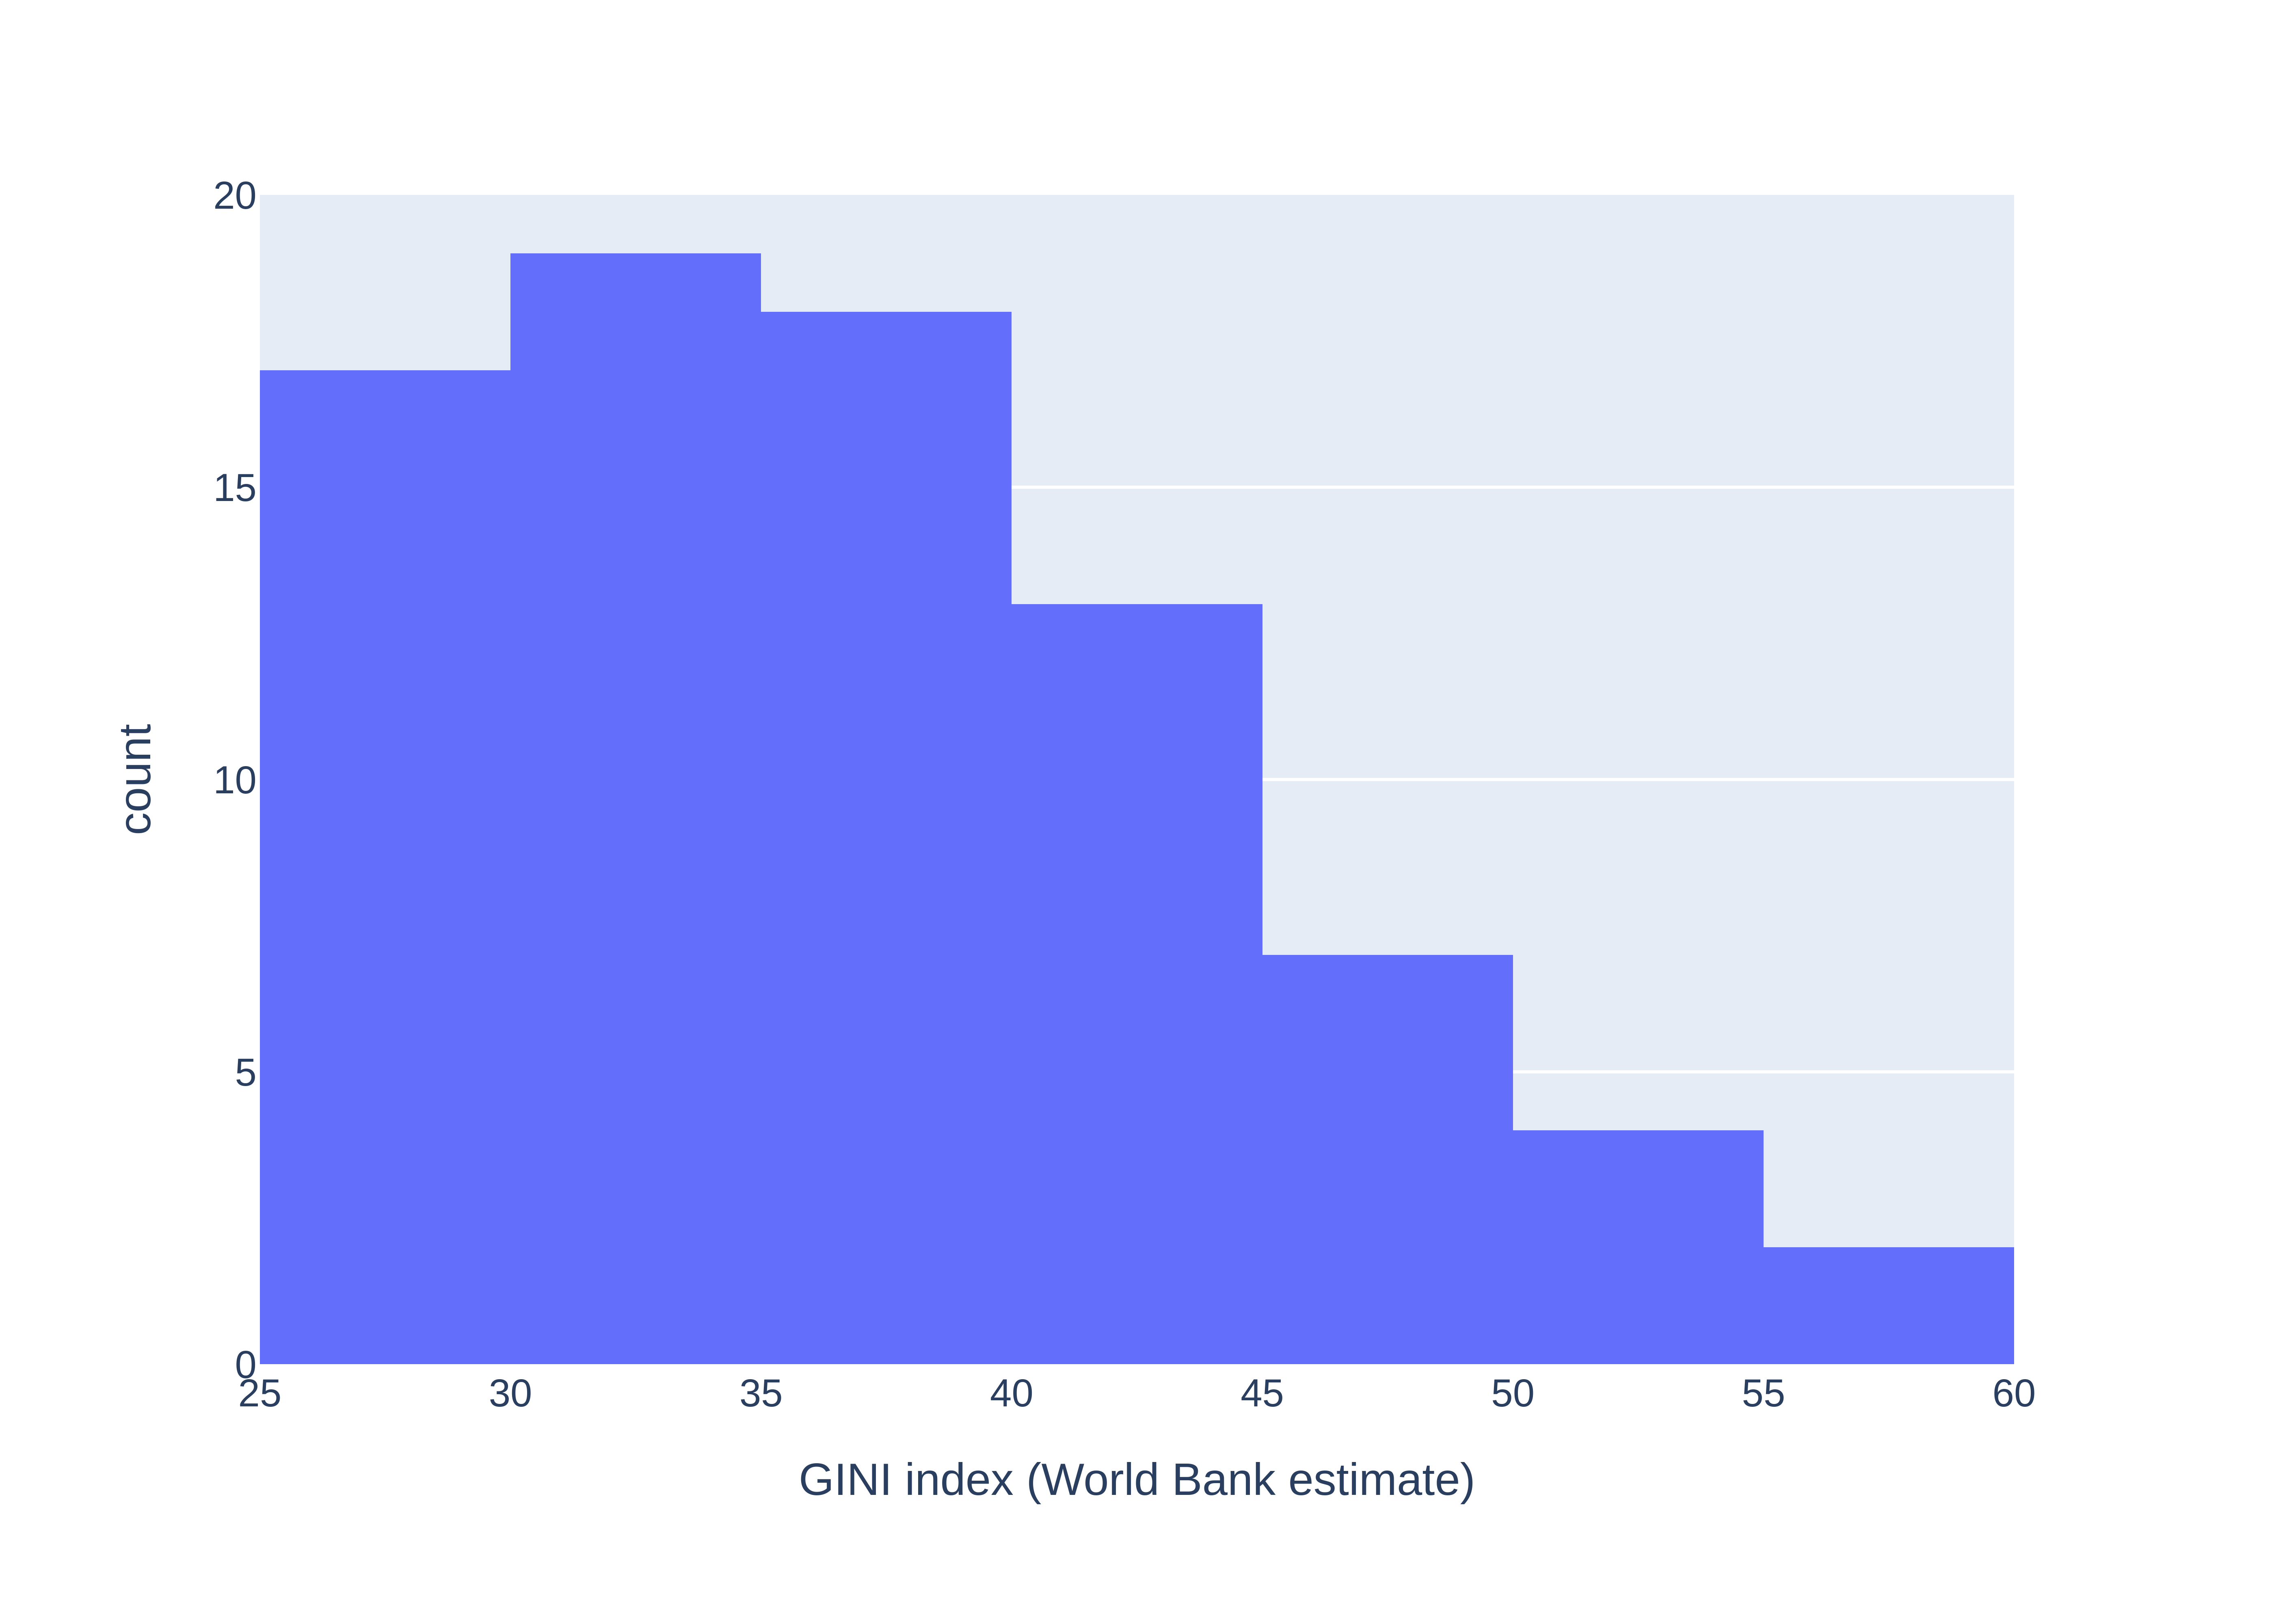
\includegraphics[width=7cm, height=7cm, keepaspectratio]{images/freq_1.png}
				\end{center}
			\end{column}
		\end{columns}
	\end{frame}
	
	\begin{frame}[fragile]{Hisztogramok felbontása}
		\begin{columns}
			\begin{column}{.5\textwidth}
				\begin{block}{Osztályköz}
					Az osztályközök határozzák meg, hogy az adatok milyen tartományokba kerülnek, és ezek az intervallumok határozzák meg a hisztogram oszlopainak szélességét.
				\end{block}
				\medskip
				Az osztályközök száma az \texttt{nbins} paraméter segítségével állítható. 
				\begin{lstlisting}[language=python]
for n in [2, 45, 500]:
	px.histogram(data_frame=df, x=gini, nbins=n)
				\end{lstlisting}
			\end{column}
			\begin{column}{.5\textwidth}
				\begin{center}
					\includegraphics<1>[width=7cm, height=7cm, keepaspectratio]{images/freq_2.png}
					\includegraphics<2>[width=7cm, height=7cm, keepaspectratio]{images/freq_3.png}
					\includegraphics<3>[width=7cm, height=7cm, keepaspectratio]{images/freq_4.png}
				\end{center}
			\end{column}
		\end{columns}
	\end{frame}
	
	\begin{frame}[fragile]{Hisztogram hasítása színekkel}
		\begin{columns}
			\begin{column}{.5\textwidth}
				Plotly express diagramokat lehetséges változón belüli csoportonként meghasítani. Ennek eléréséhez a \texttt{color} paramétert kell a megfelelő változóra állítani.\par\medskip
				\begin{lstlisting}[language=python]
px.histogram(data_frame=df, x=gini, color='Income Group', color_discrete_sequence=px.colors.qualitative.Set1)
				\end{lstlisting}
			\end{column}
			\begin{column}{.5\textwidth}
				\begin{center}
					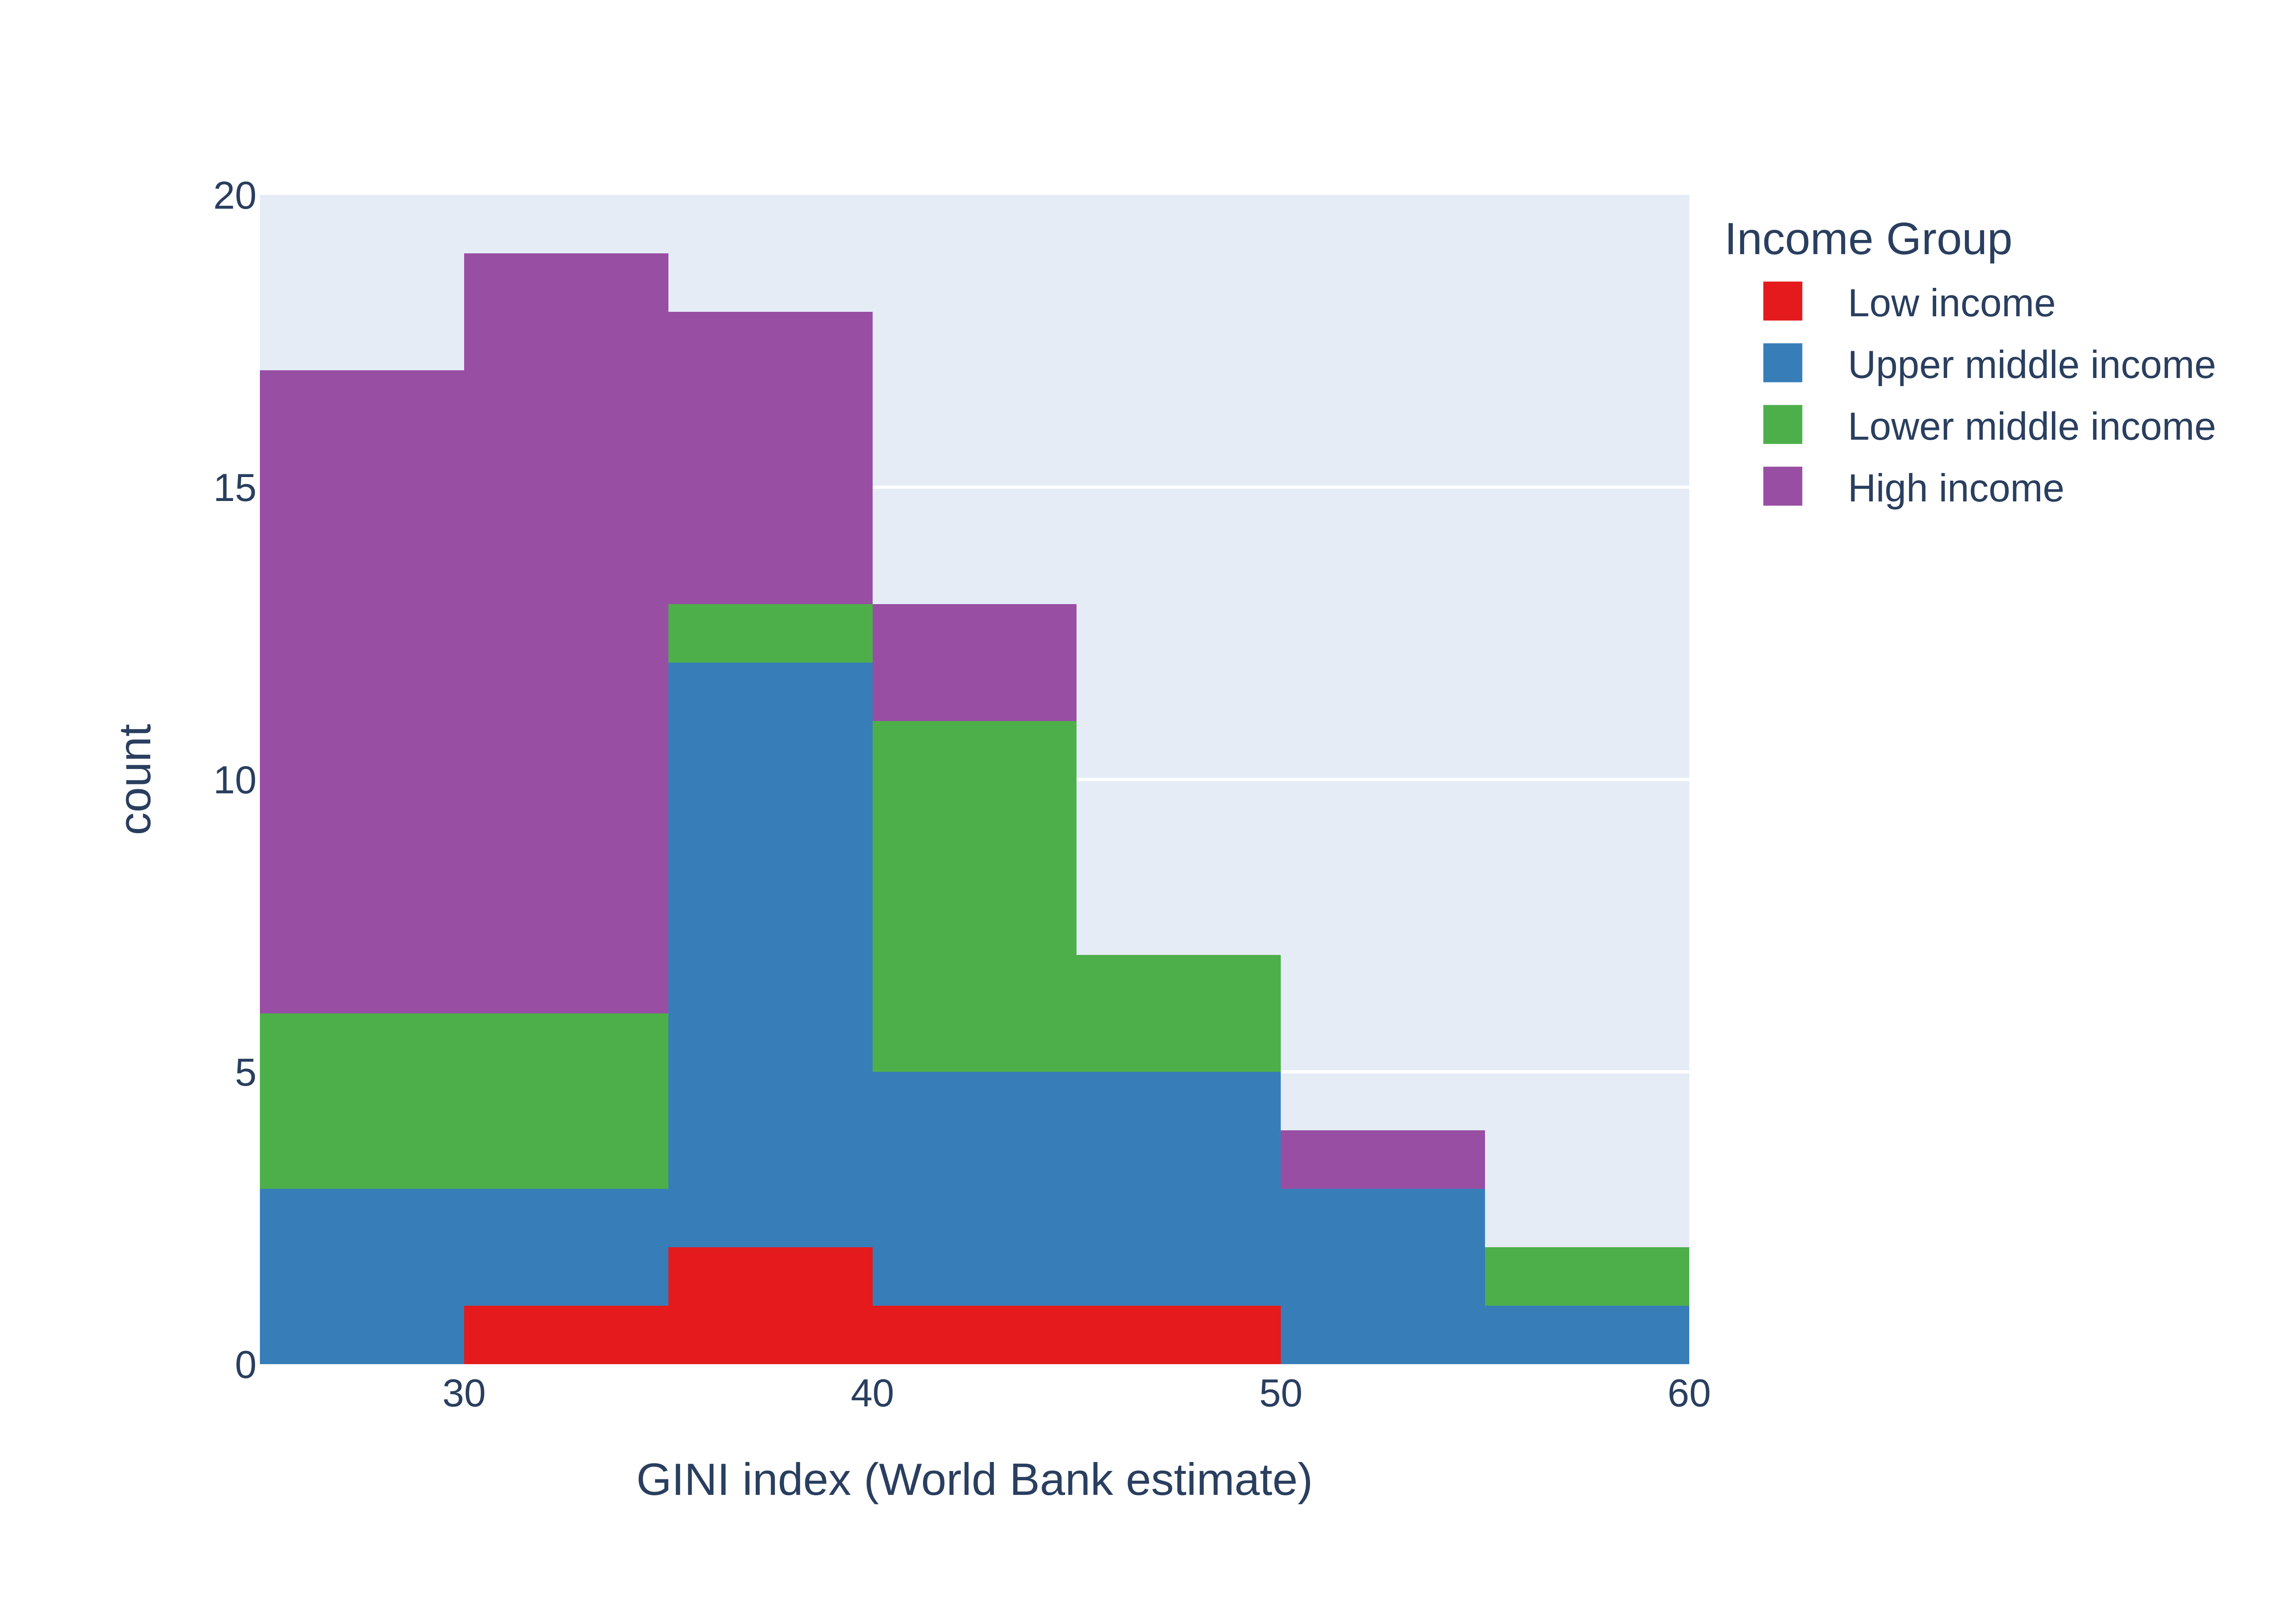
\includegraphics[width=7cm, height=7cm, keepaspectratio]{images/freq_5.png}
				\end{center}
			\end{column}
		\end{columns}
	\end{frame}
	
	\begin{frame}[fragile]{Csoportosított hisztogramok}
		\begin{columns}
			\begin{column}{.5\textwidth}
				Vannak olyan esetek, amikor egy változónak több csoportját egymás mellett szükséges megmutatni. Ekkor a hisztogramokat lehetséges csoportosítani adott értékek szerint, a \texttt{color} és a \texttt{barmode='group'} paraméterek állításával.\par\medskip
				\begin{lstlisting}[language=python]
px.histogram(df, x=gini, color='year', barmode='group')
				\end{lstlisting}
			\end{column}
			\begin{column}{.5\textwidth}
				\begin{center}
					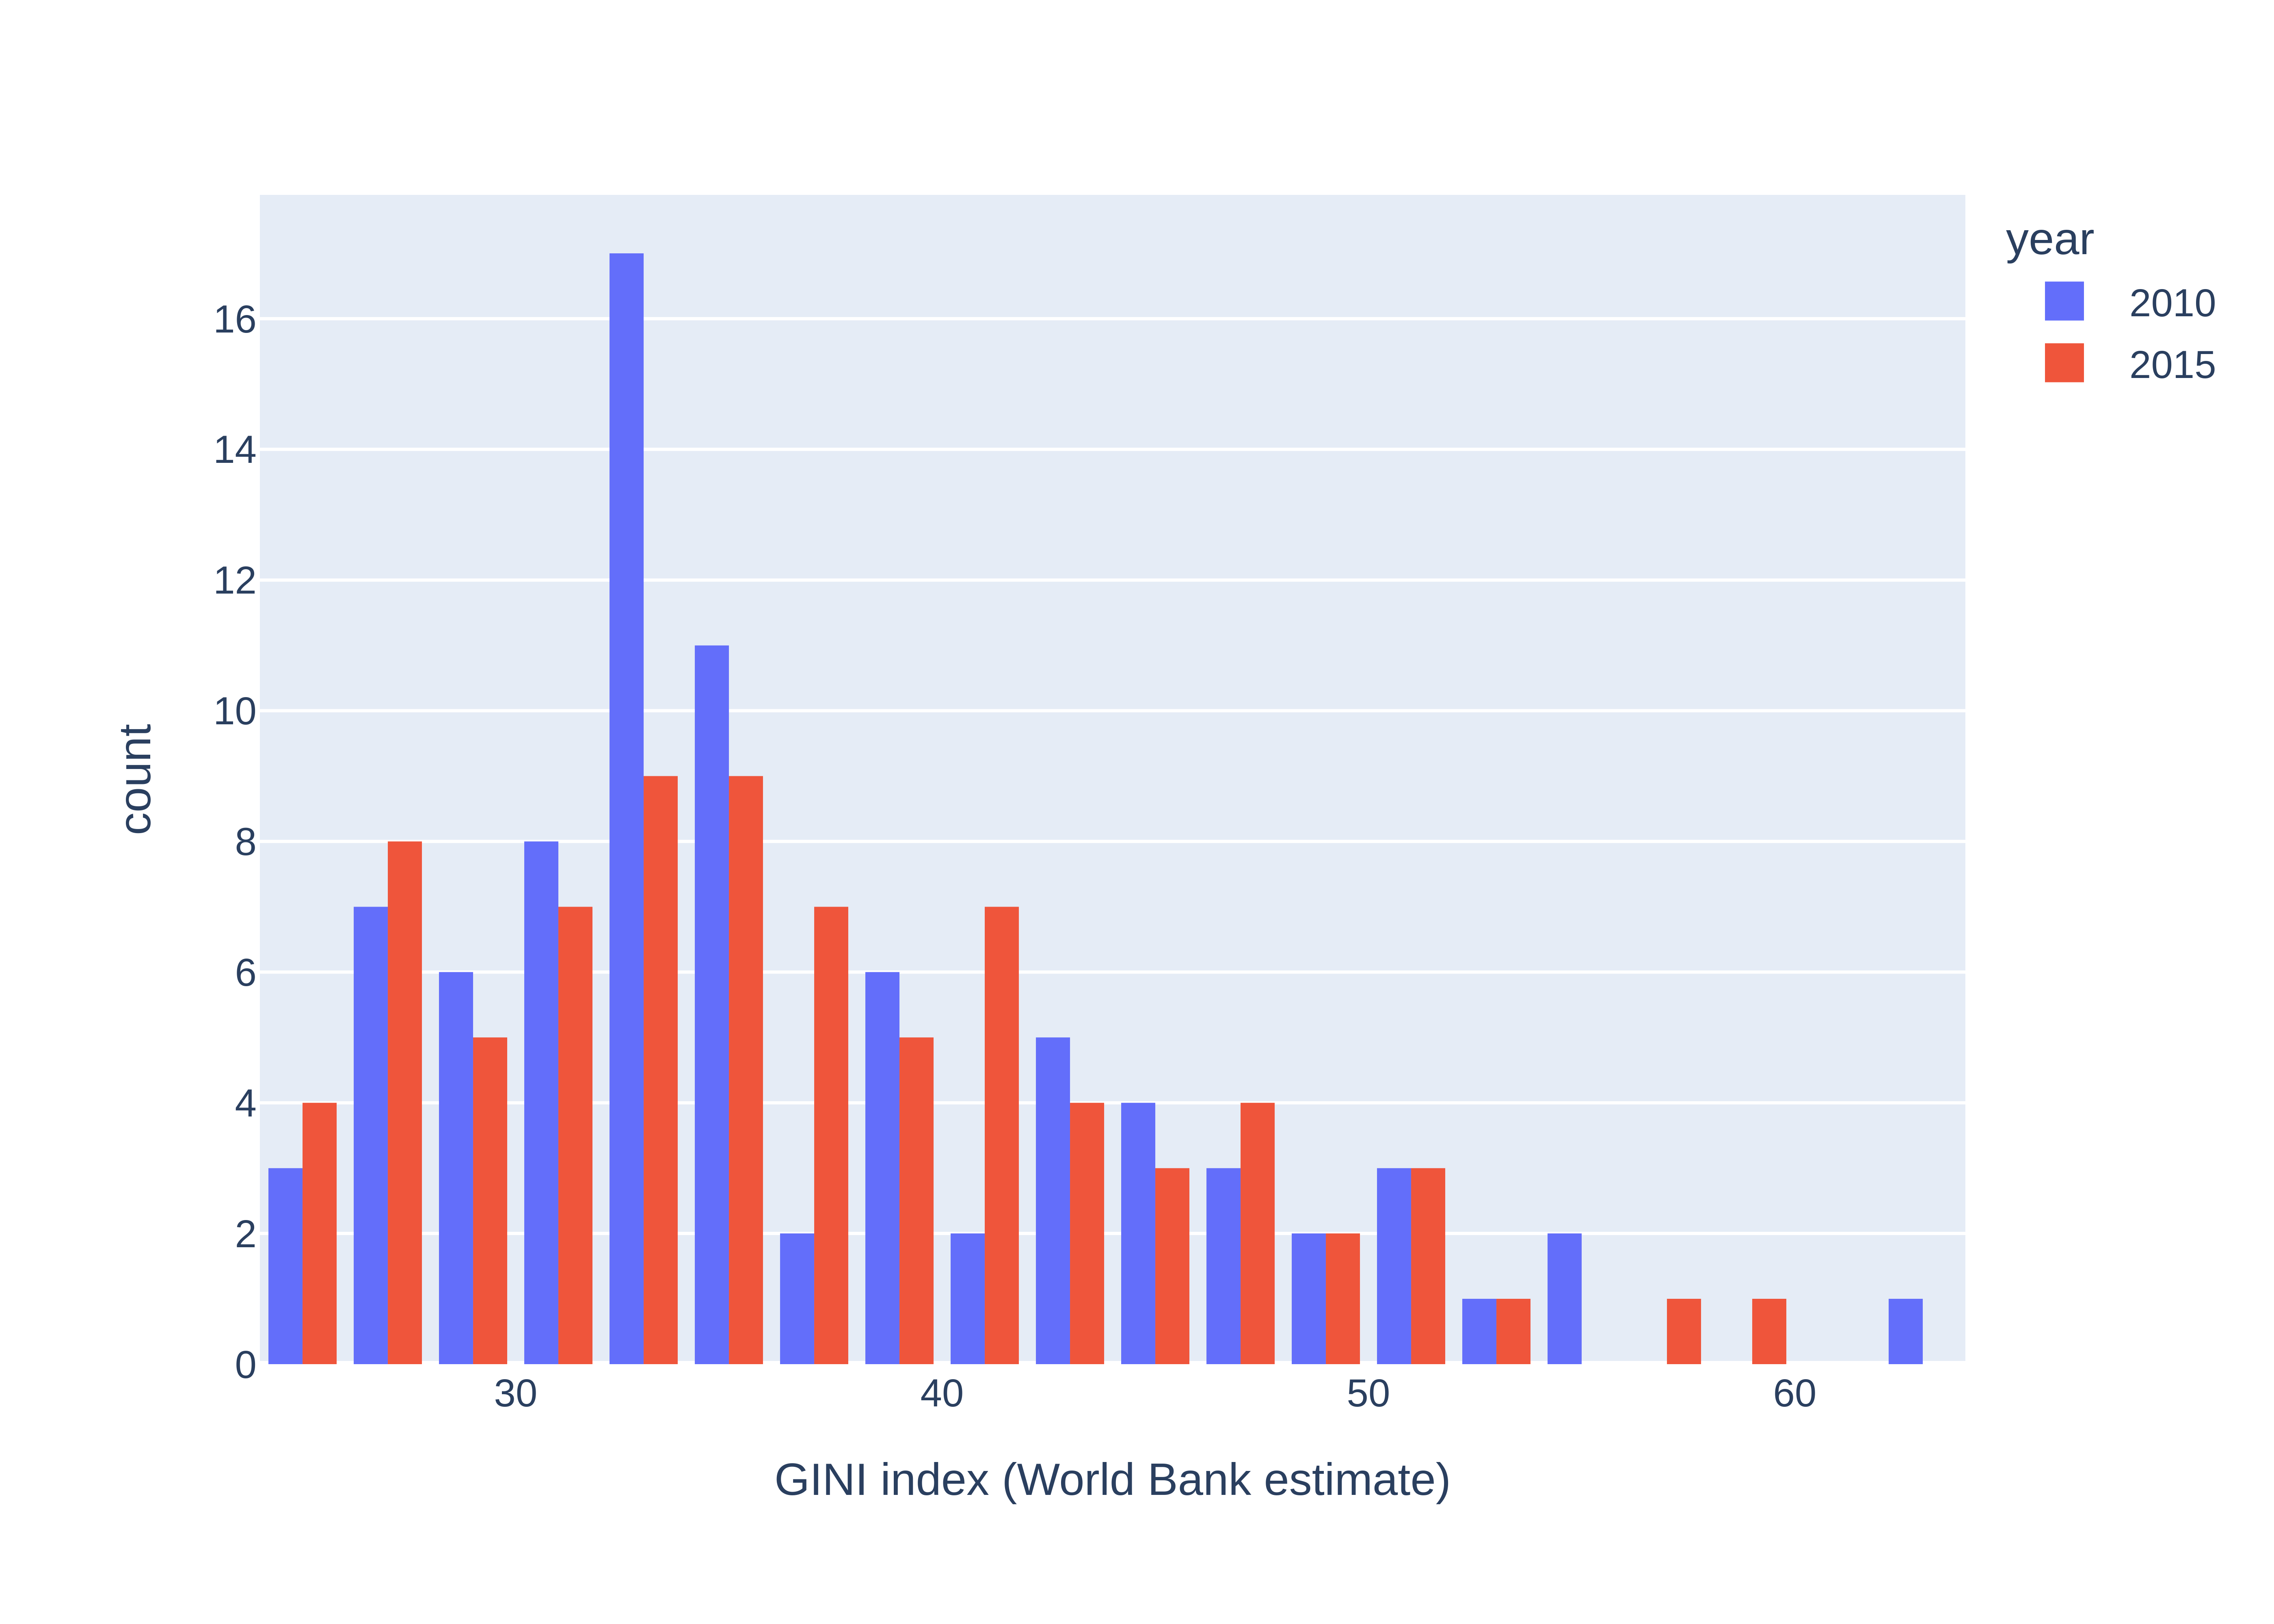
\includegraphics[width=7cm, height=7cm, keepaspectratio]{images/freq_6.png}
				\end{center}
			\end{column}
		\end{columns}
	\end{frame}
	
	\begin{frame}[fragile]{Hasított hisztogramok}
		\begin{columns}
			\begin{column}{.5\textwidth}
				A diagramok hasítása adott változó értékei szerint lehetséges úgy is, hogy minden, a változóhoz tartozó értékre szűrt adathalmaz egy külön diagramon jelenik meg, a \texttt{facet\_col} paraméter állításával.\par\medskip
				\begin{lstlisting}[language=python]
px.histogram(df, x=gini, color='year', facet_col='year')
				\end{lstlisting}
			\end{column}
			\begin{column}{.5\textwidth}
				\begin{center}
					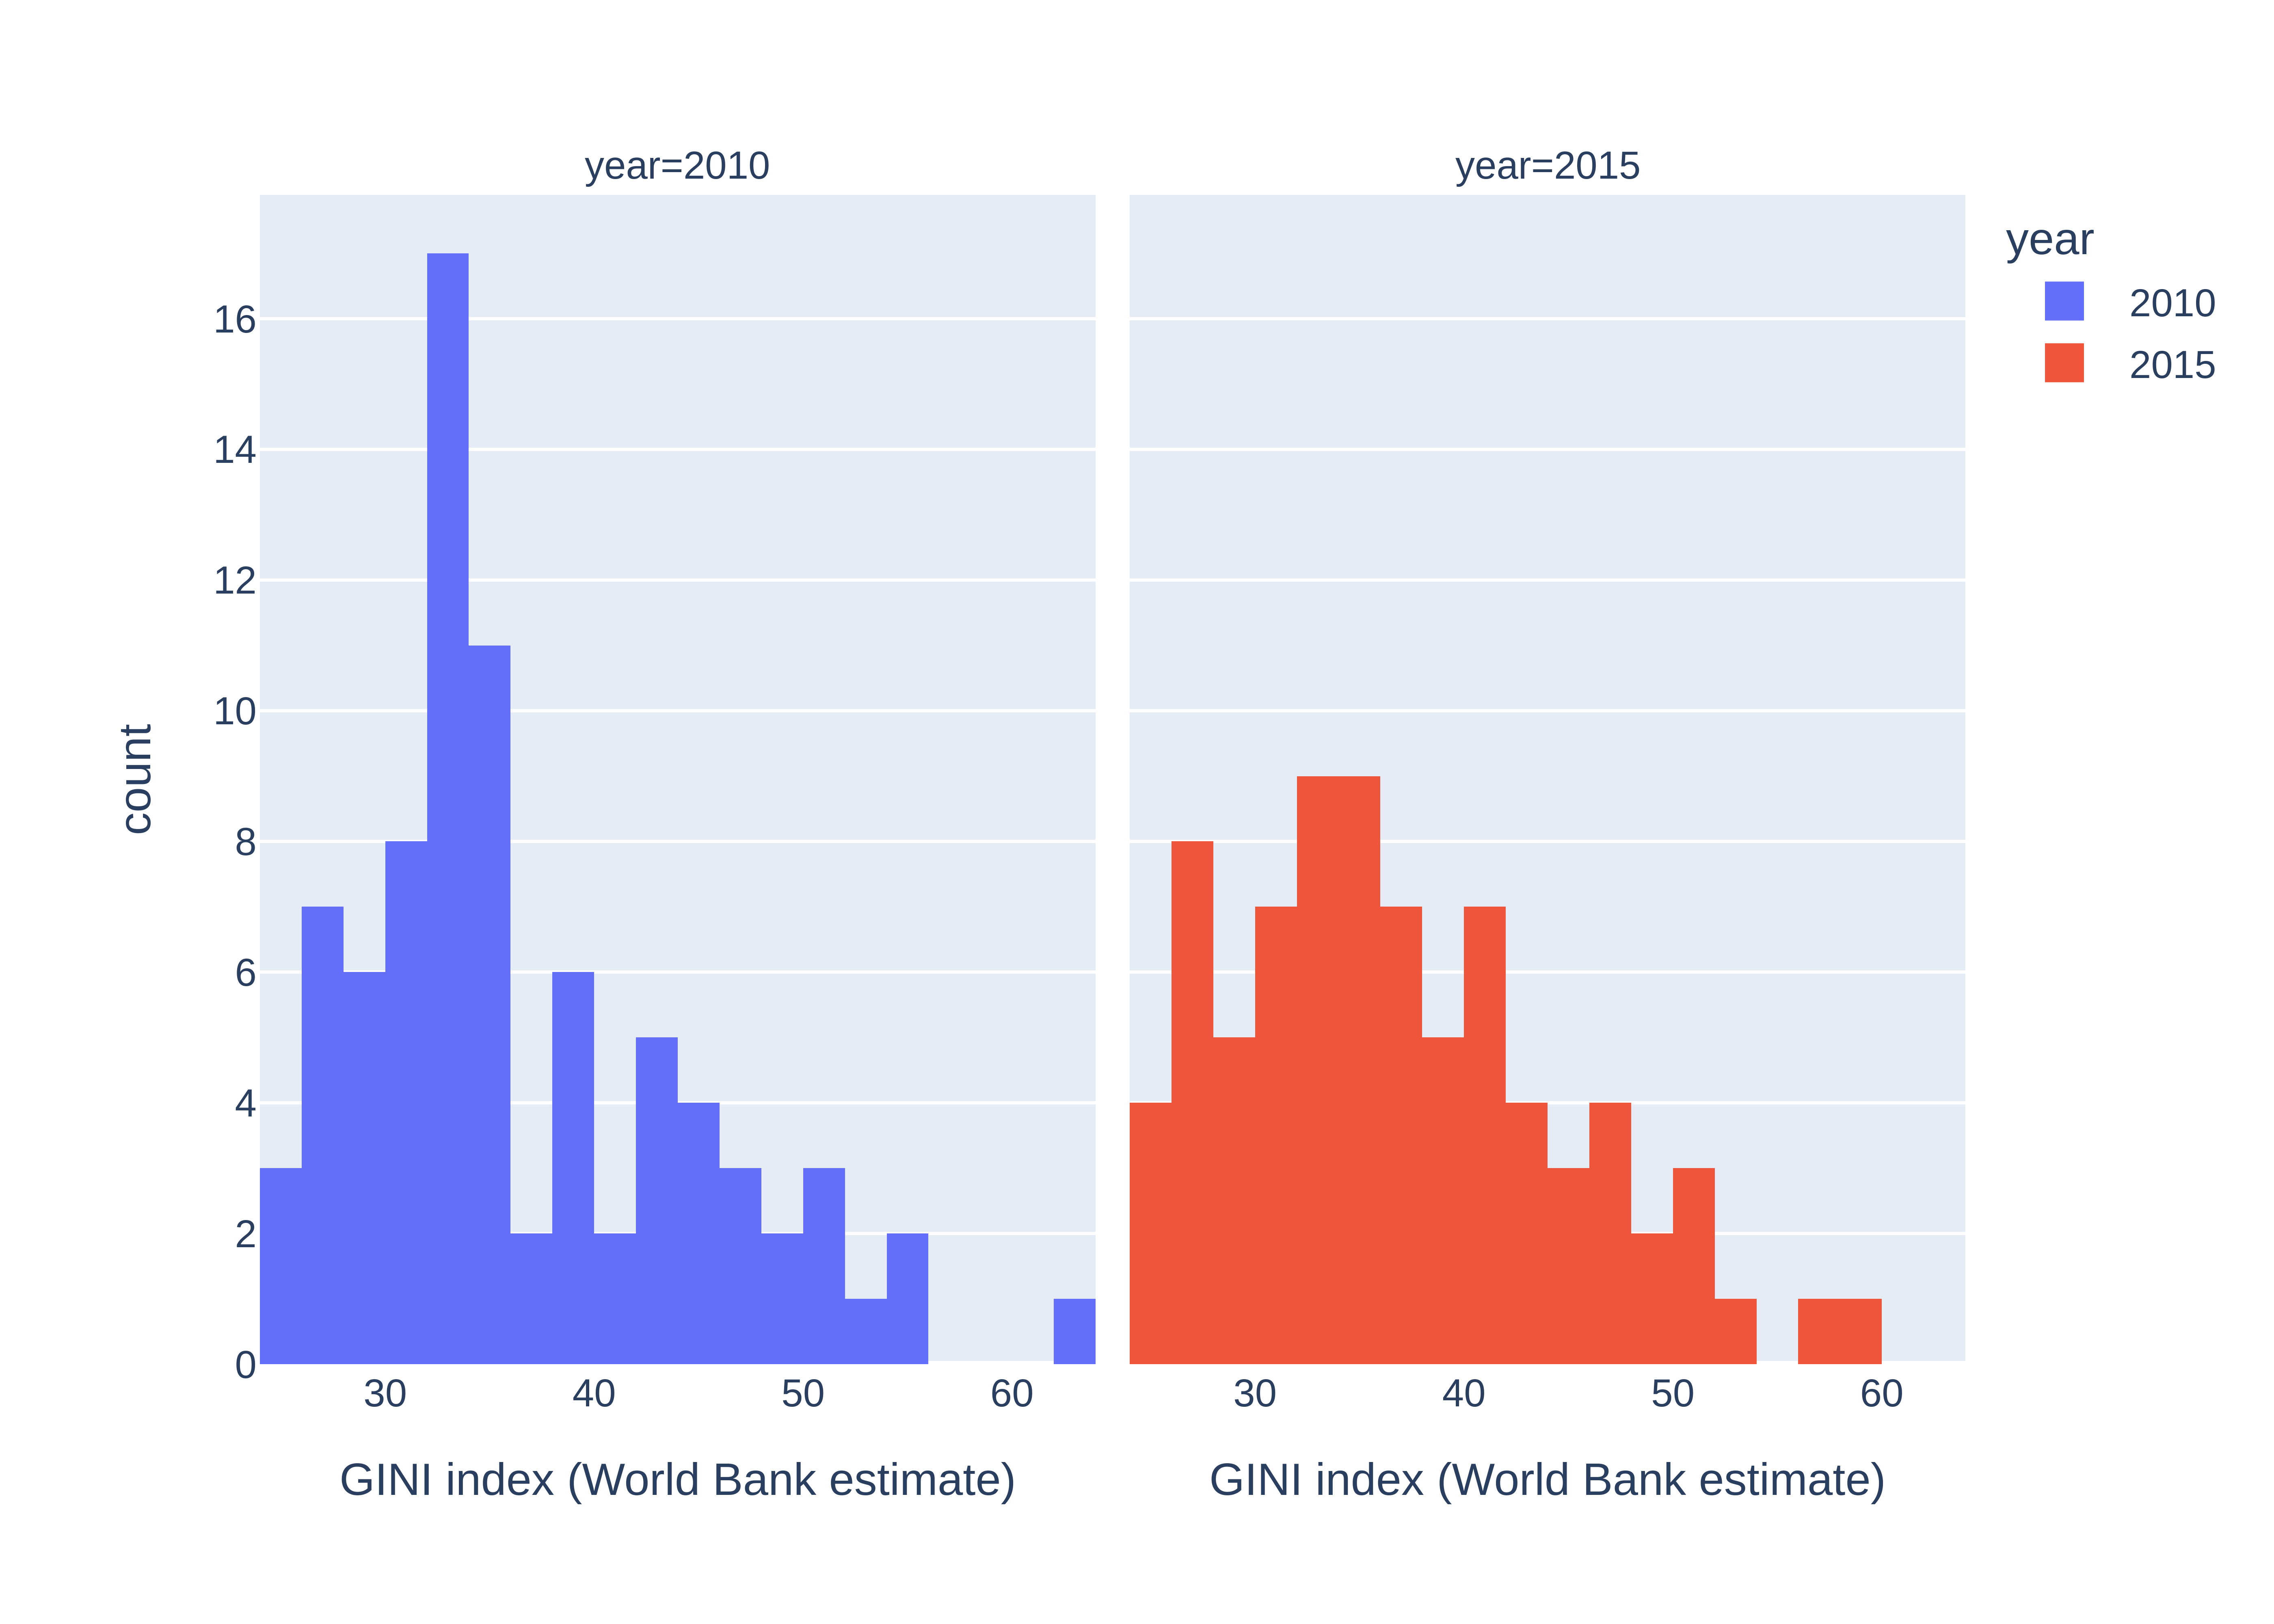
\includegraphics[width=7cm, height=7cm, keepaspectratio]{images/freq_7.png}
				\end{center}
			\end{column}
		\end{columns}
	\end{frame}
	
	\begin{frame}[fragile]{Hisztogramok normalizálása}
		\begin{columns}
			\begin{column}{.5\textwidth}
				\begin{block}{Normalizált hisztogram}
					Olyan grafikon, ahol az egyes oszlopok az adott intervallumba eső adatok gyakoriságát jelzi olyan módon, hogy az oszlopok összege 1 legyen. 
				\end{block}
				\begin{lstlisting}[language=python]
fig = px.histogram(df, x=gini, color='year', facet_col='year')
fig.layout.yaxis.ticksuffix = '%'
fig.layout.yaxis.title = 'Százalékos gyakoriság'
fig.show()
				\end{lstlisting}
			\end{column}
			\begin{column}{.5\textwidth}
				\begin{center}
					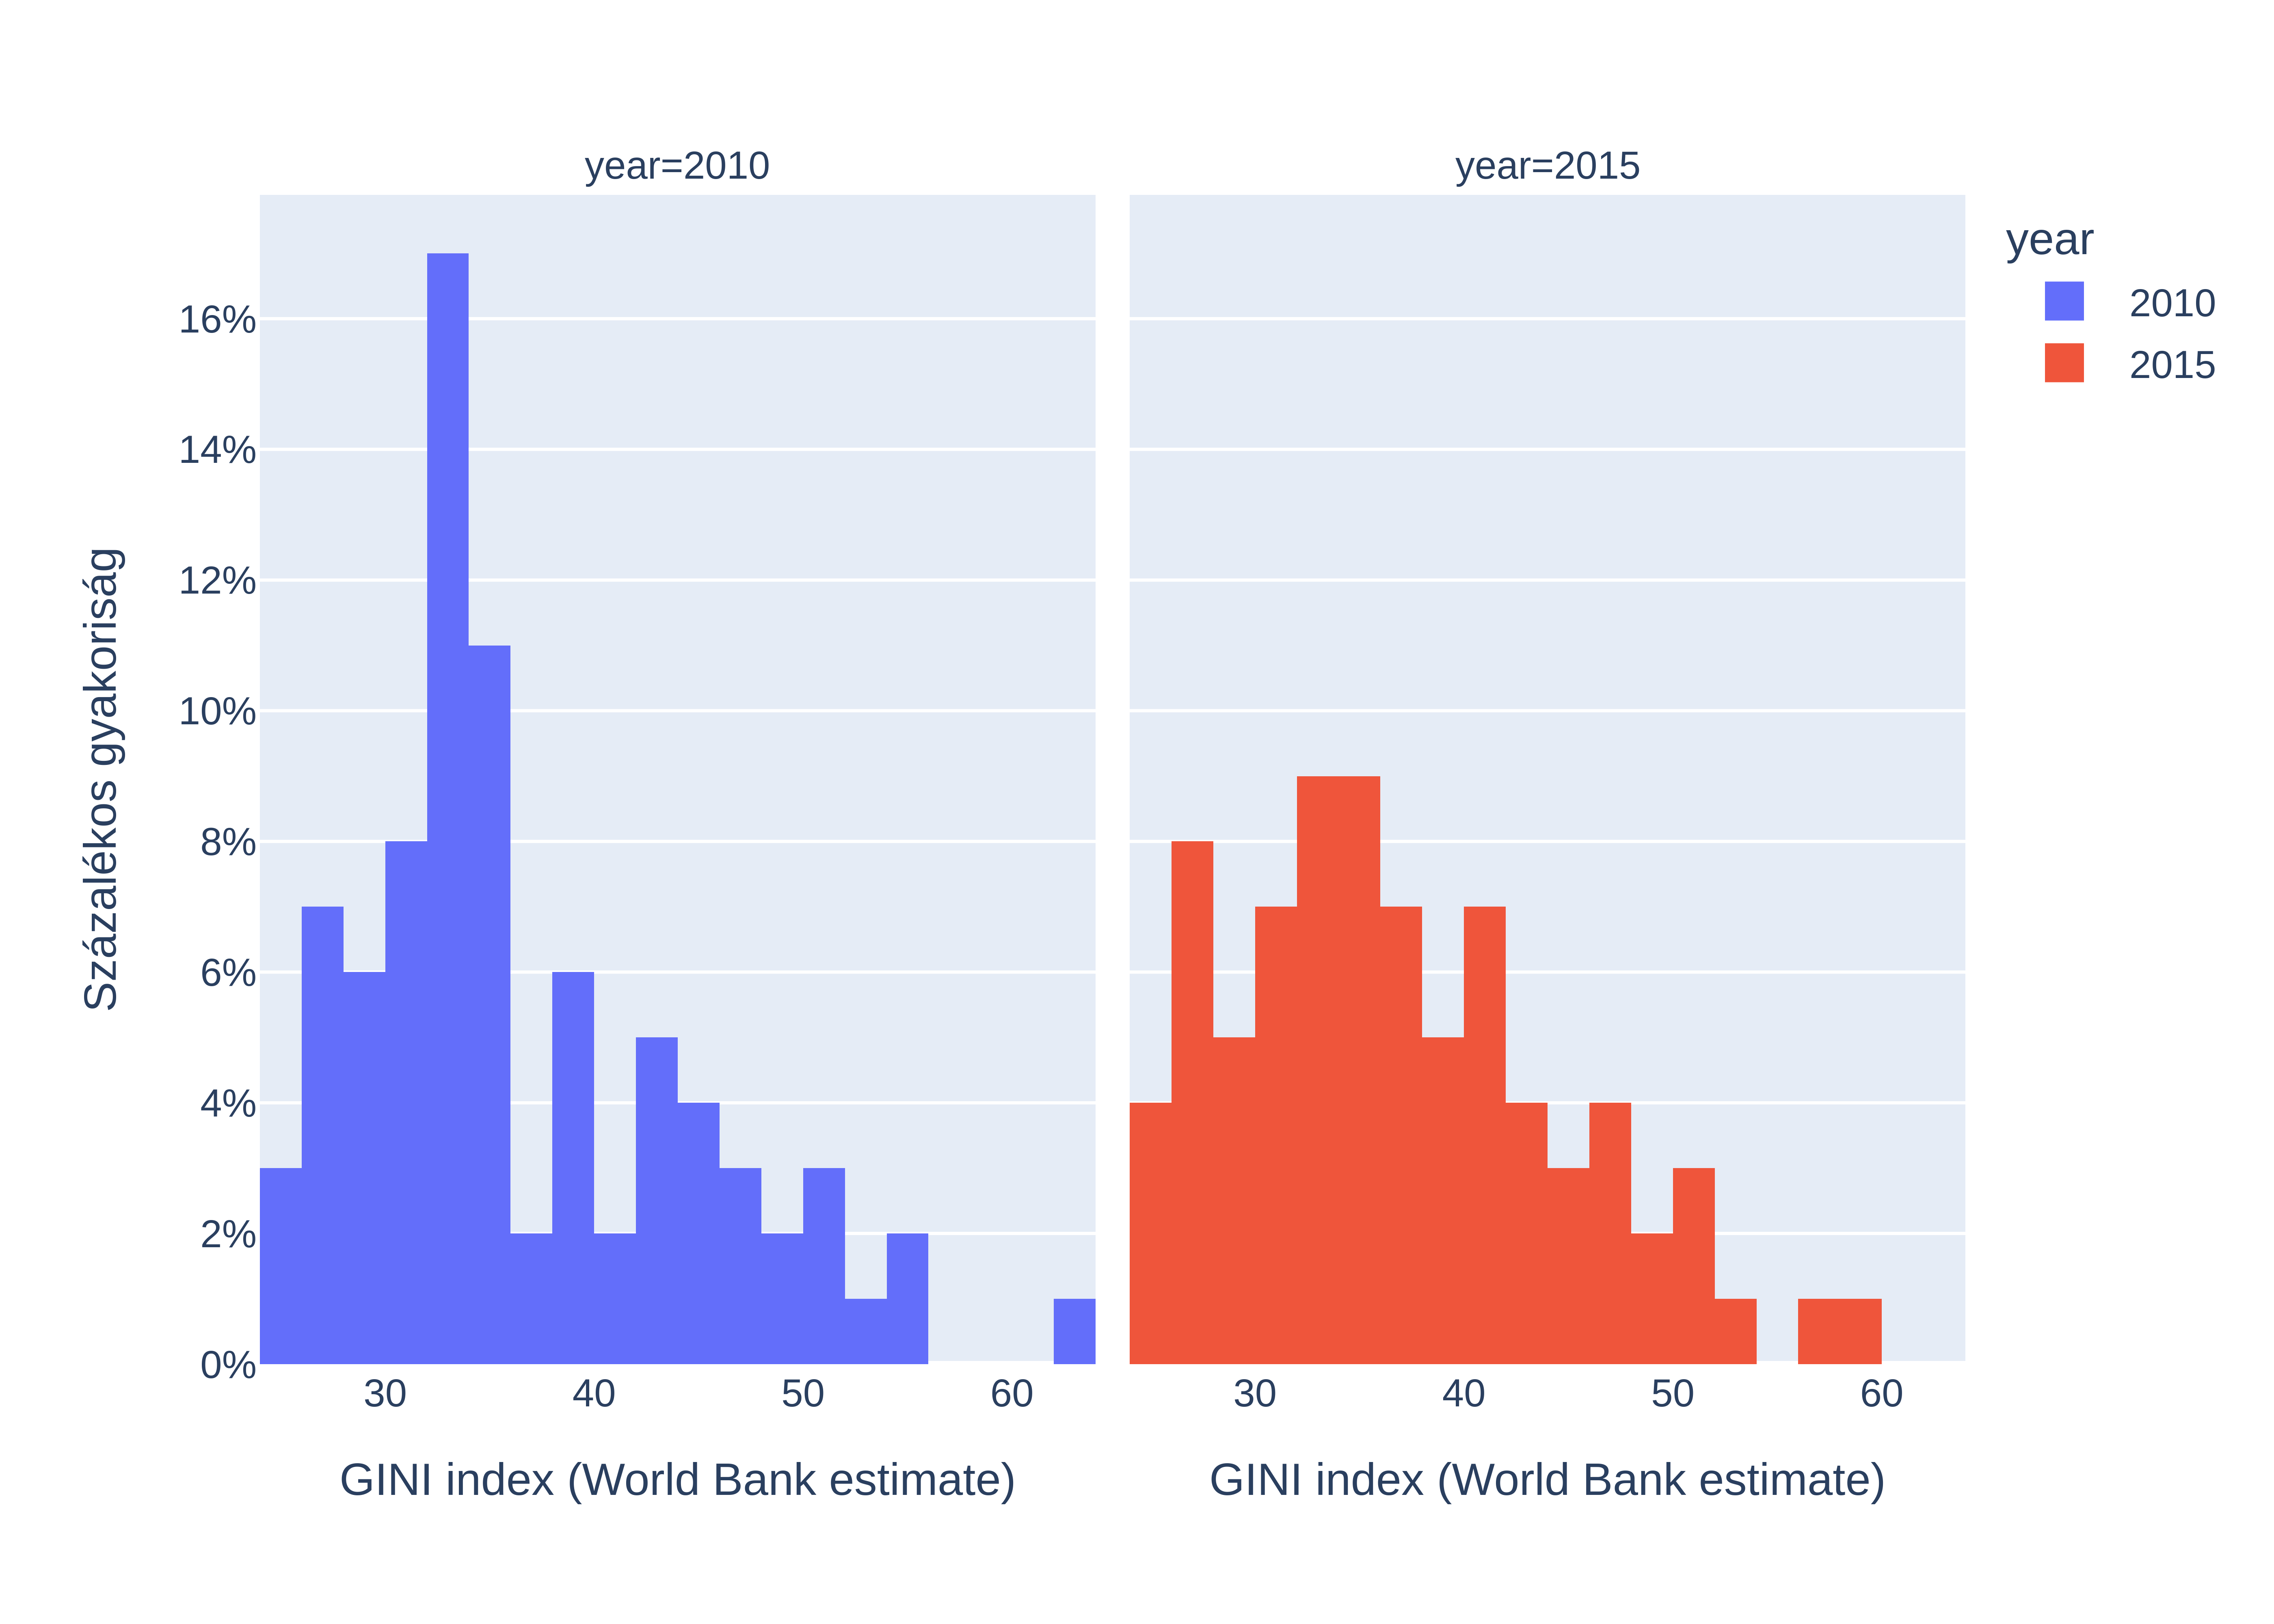
\includegraphics[width=7cm, height=7cm, keepaspectratio]{images/freq_8.png}
				\end{center}
			\end{column}
		\end{columns}
	\end{frame}
	
	\begin{frame}[fragile]{Hisztogramok több dimenzióban}
		\begin{columns}
			\begin{column}{.5\textwidth}
				\begin{block}{2D hisztogram}
					Két dimenzióban osztja fel az adatokat, és minden cella (osztályköz) azt mutatja meg, hogy hány adatpont esik az adott tartományba mindkét változó esetében. 
				\end{block}
				\begin{lstlisting}[language=python]
fig = go.Figure()
fig.add_histogram2d(
	x=df['Income share held by fourth 20%'],
	y=df['GINI index (World Bank estimate)'],
	colorscale='cividis'
)
				\end{lstlisting}
			\end{column}
			\begin{column}{.5\textwidth}
				\begin{center}
					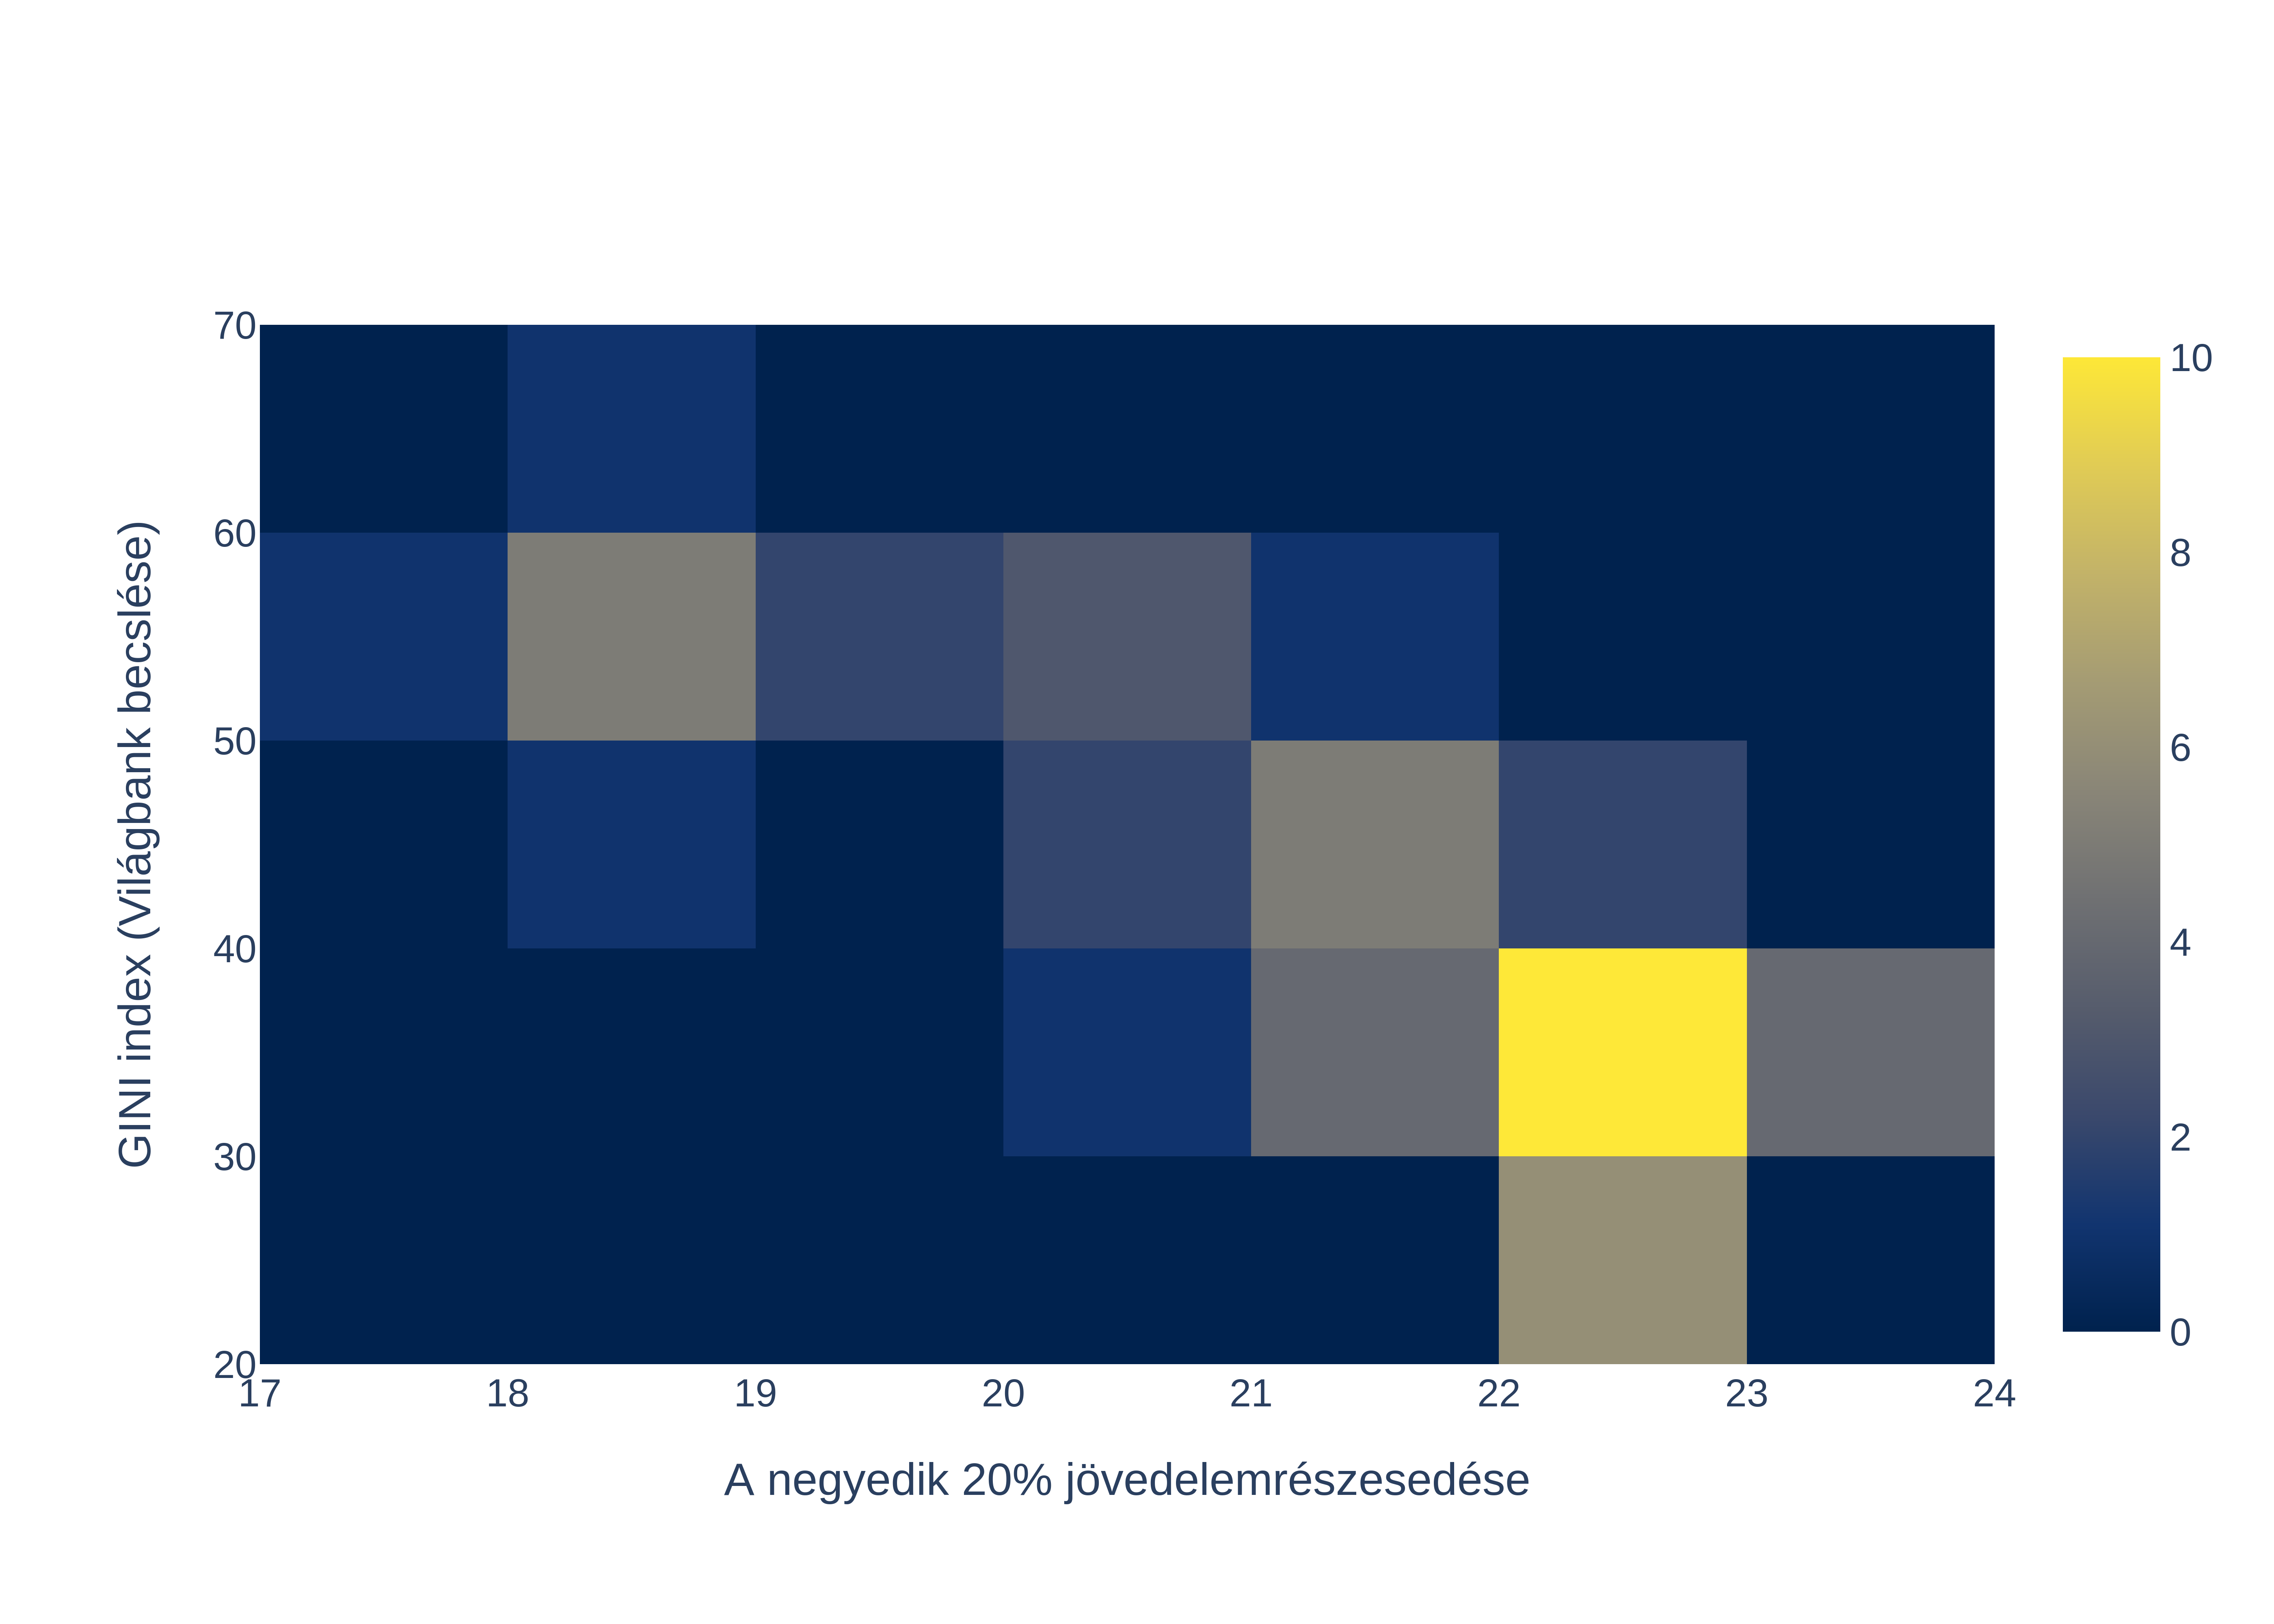
\includegraphics[width=7cm, height=7cm, keepaspectratio]{images/freq_11.png}
				\end{center}
			\end{column}
		\end{columns}
	\end{frame}
	
	\begin{frame}{Alkalmazás interaktív hisztogramokkal (\texttt{freq\_app\_v1.py})}
		\begin{columns}
			\begin{column}{.5\textwidth}
				A callback függvények a felhasználói interakciók alapján frissítik a grafikonokat. A \texttt{display\_histogram} függvény három bemeneti elemet figyel \texttt{(years, indicator, bins)}, és ezek alapján frissíti a hisztogram ábrát.\par\medskip
				Ha nincs kiválasztott év vagy indikátor, a függvény nem frissíti az ábrát (\texttt{PreventUpdate}). Az adatok szűrése után a Plotly Express segítségével készül el a hisztogram.
			\end{column}
			\begin{column}{.5\textwidth}
				\begin{center}
					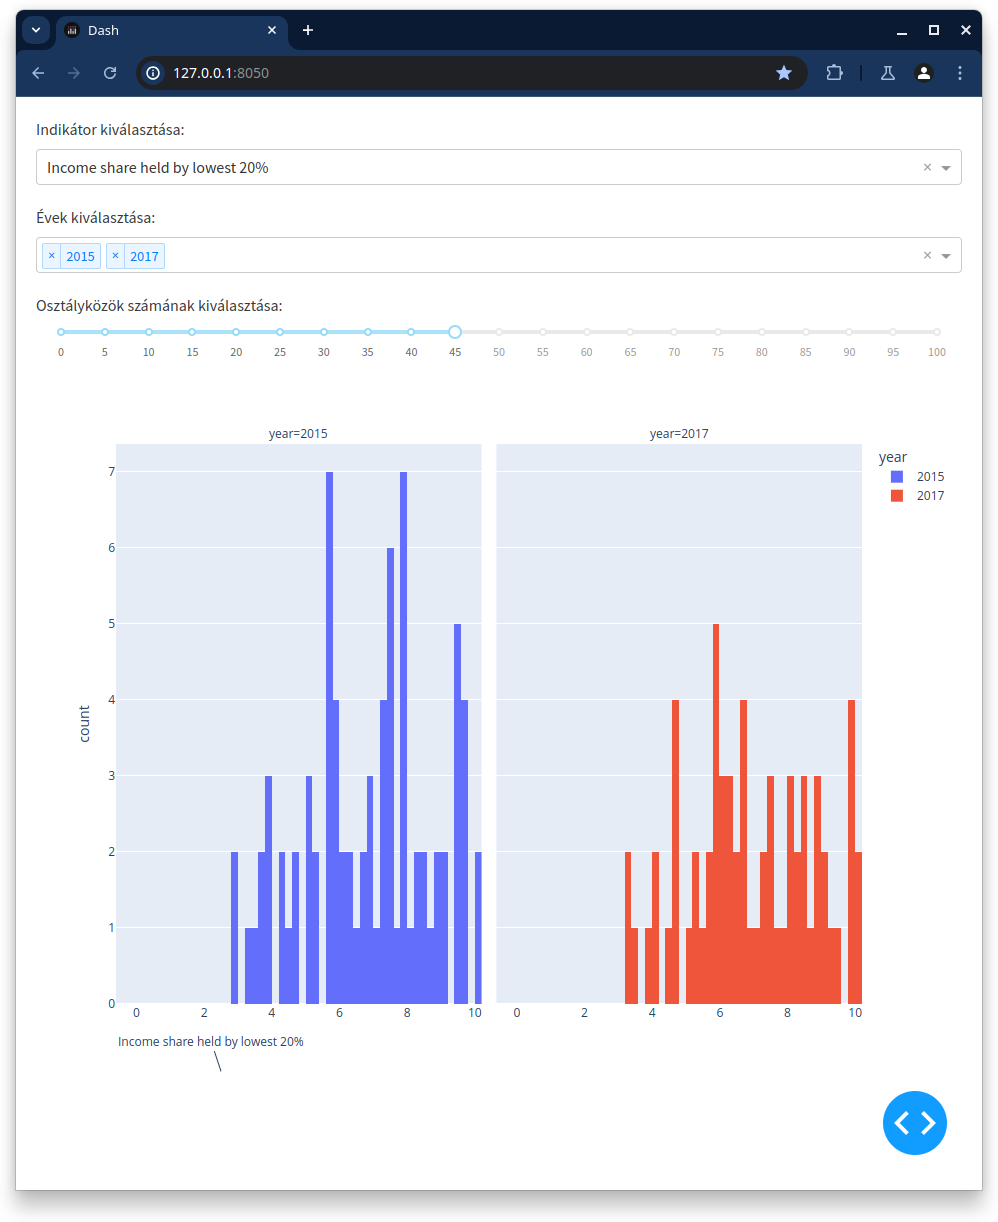
\includegraphics[width=7cm, height=7cm, keepaspectratio]{images/freq_9.png}
				\end{center}
			\end{column}
		\end{columns}
	\end{frame}
	
	\begin{frame}{Interaktív hisztogramok beépítése az alkalmazásba (\texttt{app\_v4\_1.py})}
		\begin{center}
			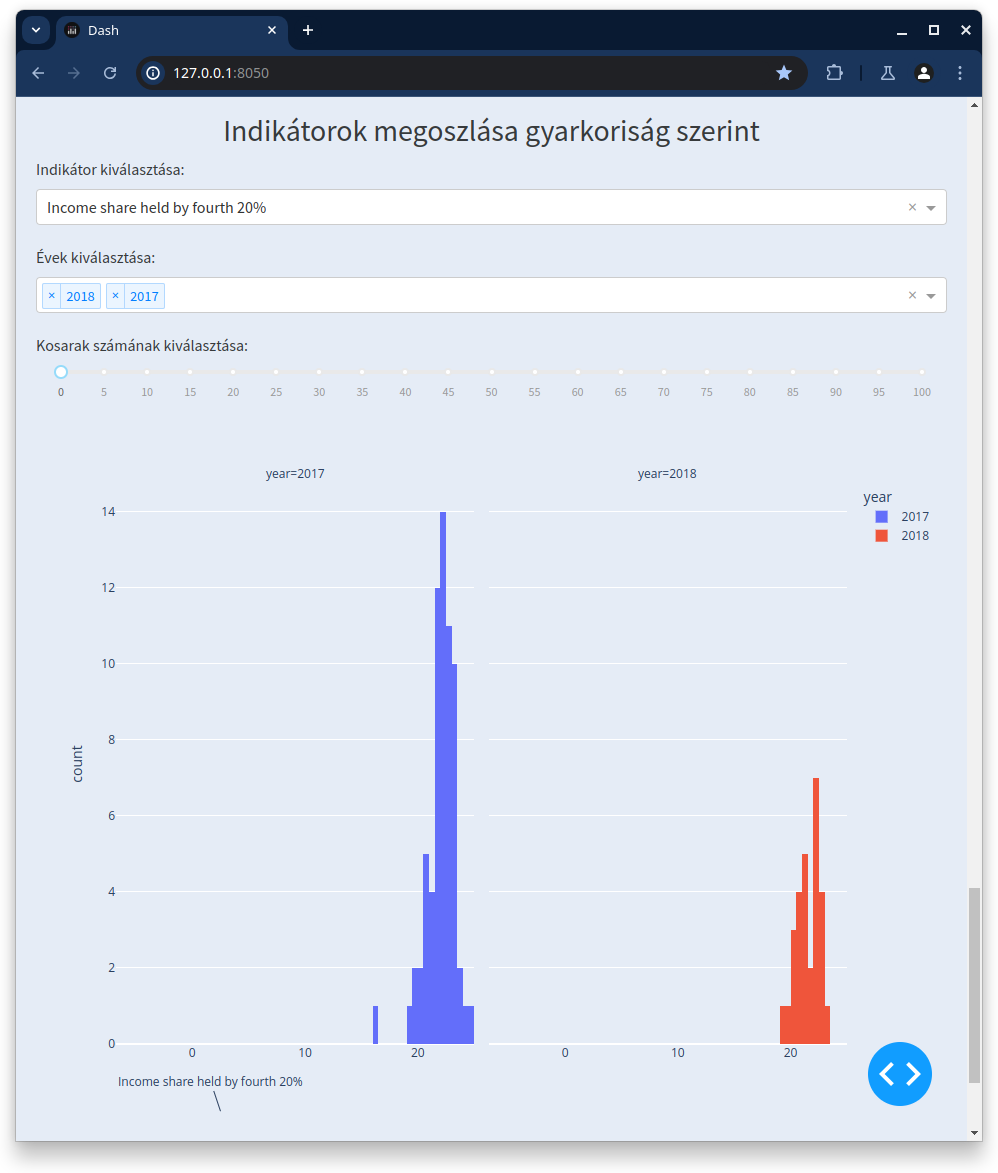
\includegraphics[width=7cm, height=7cm, keepaspectratio]{images/freq_10.png}
		\end{center}
	\end{frame}
	
	\section{Adattáblák}
	
	\begin{frame}{}
		\tableofcontents[currentsection]
	\end{frame}
	
	\begin{frame}[fragile]{Adattábla létrehozása}
		\begin{columns}
			\begin{column}{.5\textwidth}
				A Dash keretrendszerben interaktív táblázatokat a \texttt{dash\_table} könyvtárral lehet létrehozni.\par\medskip
				\begin{lstlisting}[language=python]
from dash import html, dash_table

app.layout = html.Div([
	...
	dash_table.DataTable(
		data=pov_df.to_dict('records'),
		columns=[{'name': col, 'id': col} for col in pov_df.columns]
	)
	...
])
	
				\end{lstlisting}
			\end{column}
			\begin{column}{.5\textwidth}
				\begin{center}
					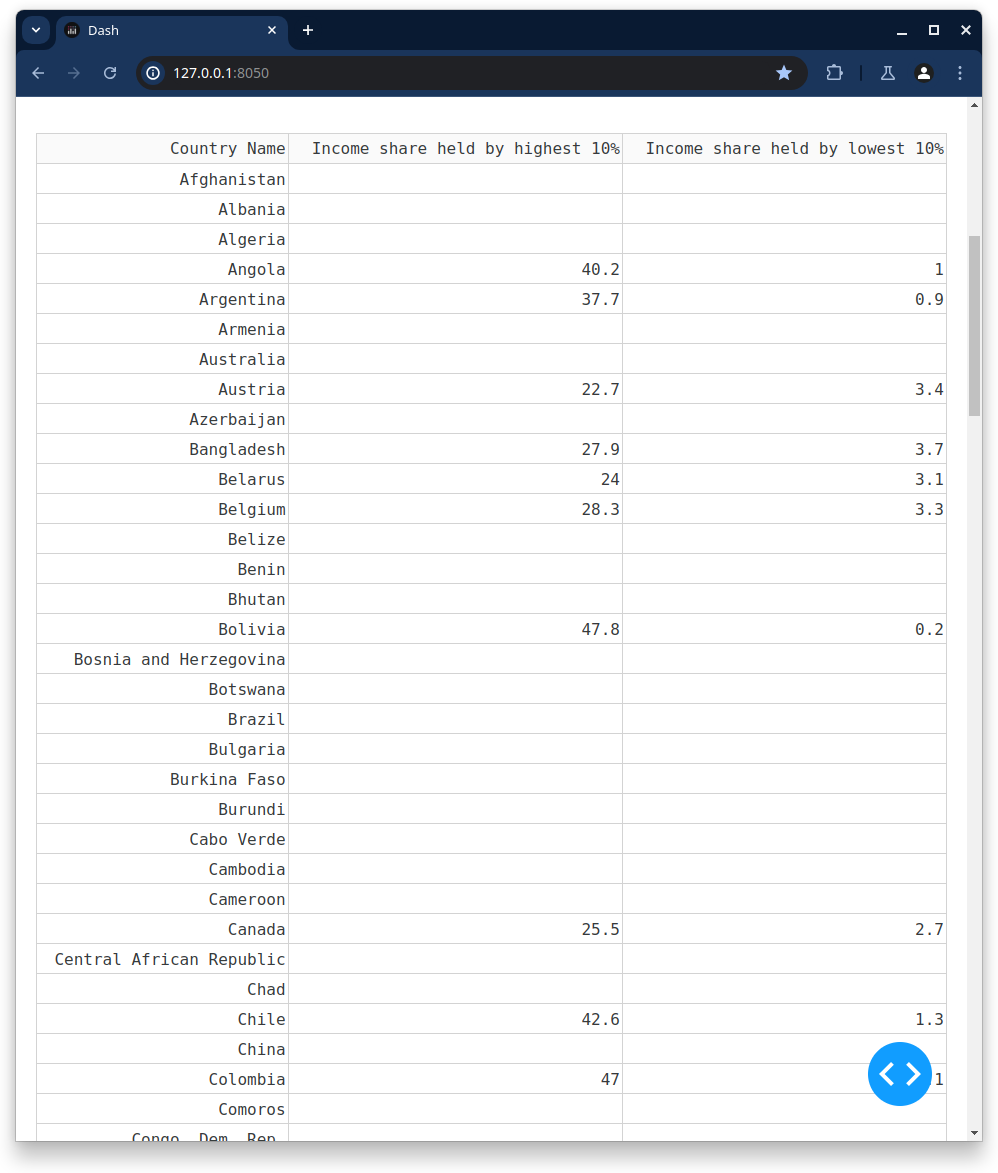
\includegraphics[width=7cm, height=7cm, keepaspectratio]{images/freq_12.png}
				\end{center}
			\end{column}
		\end{columns}
	\end{frame}
	
	\begin{frame}[fragile]{Adattábla személyre szabása}
		\begin{columns}
			\begin{column}{.5\textwidth}
				\begin{lstlisting}[language=python]
dash_table.DataTable(
	data=pov_df.to_dict('records'),
	columns=[{'name': col, 'id': col} for col in pov_df.columns],
	style_header={'whiteSpace': 'normal'},
	fixed_rows={'headers': True},
	style_table={'height': '400px'},
	virtualization=True,   
)
				\end{lstlisting}
			\end{column}
			\begin{column}{.5\textwidth}
				\begin{center}
					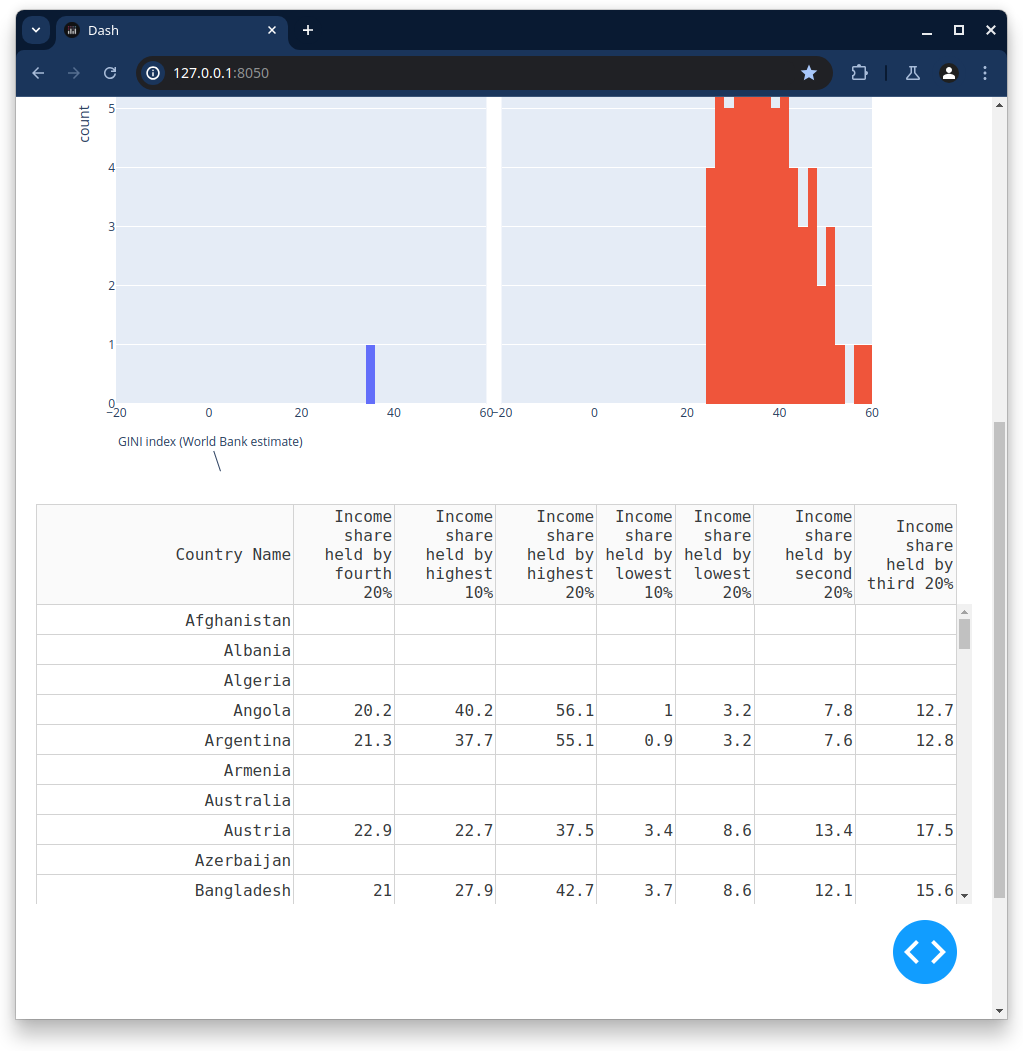
\includegraphics[width=7cm, height=7cm, keepaspectratio]{images/freq_13.png}
				\end{center}
			\end{column}
		\end{columns}
	\end{frame}
	
	\section{Gépi tanulás}
	
	\begin{frame}{}
		\tableofcontents[currentsection]
	\end{frame}
	
	\begin{frame}{$K$-közép klaszterezés}
		\begin{columns}
			\begin{column}{.5\textwidth}
				Az algoritmus eljárása:
				\begin{enumerate}
					\item $K$ számú klaszter centroid inicializálása véletlenszerűen: $\mu_1, \mu_2, \ldots, \mu_K$
					\item Minden $x_i$ adatpont a hozzá legközelebb eső klaszterhez rendelése az euklideszi távolságot használva: $c_i = \arg\min_{j} \left\| x_i - \mu_j \right\|^2$
					\item Klaszterközéppontok újraszámítása úgy, hogy az adott klaszterhez tartozó pontok várható értékét tükrözzék: $\mu_j = \frac{1}{|C_j|} \sum_{x_i \in C_j} x_i$
					\item Ismétlés a kilépési kritériumig
				\end{enumerate}
			\end{column}
			\begin{column}{.5\textwidth}
				\begin{center}
					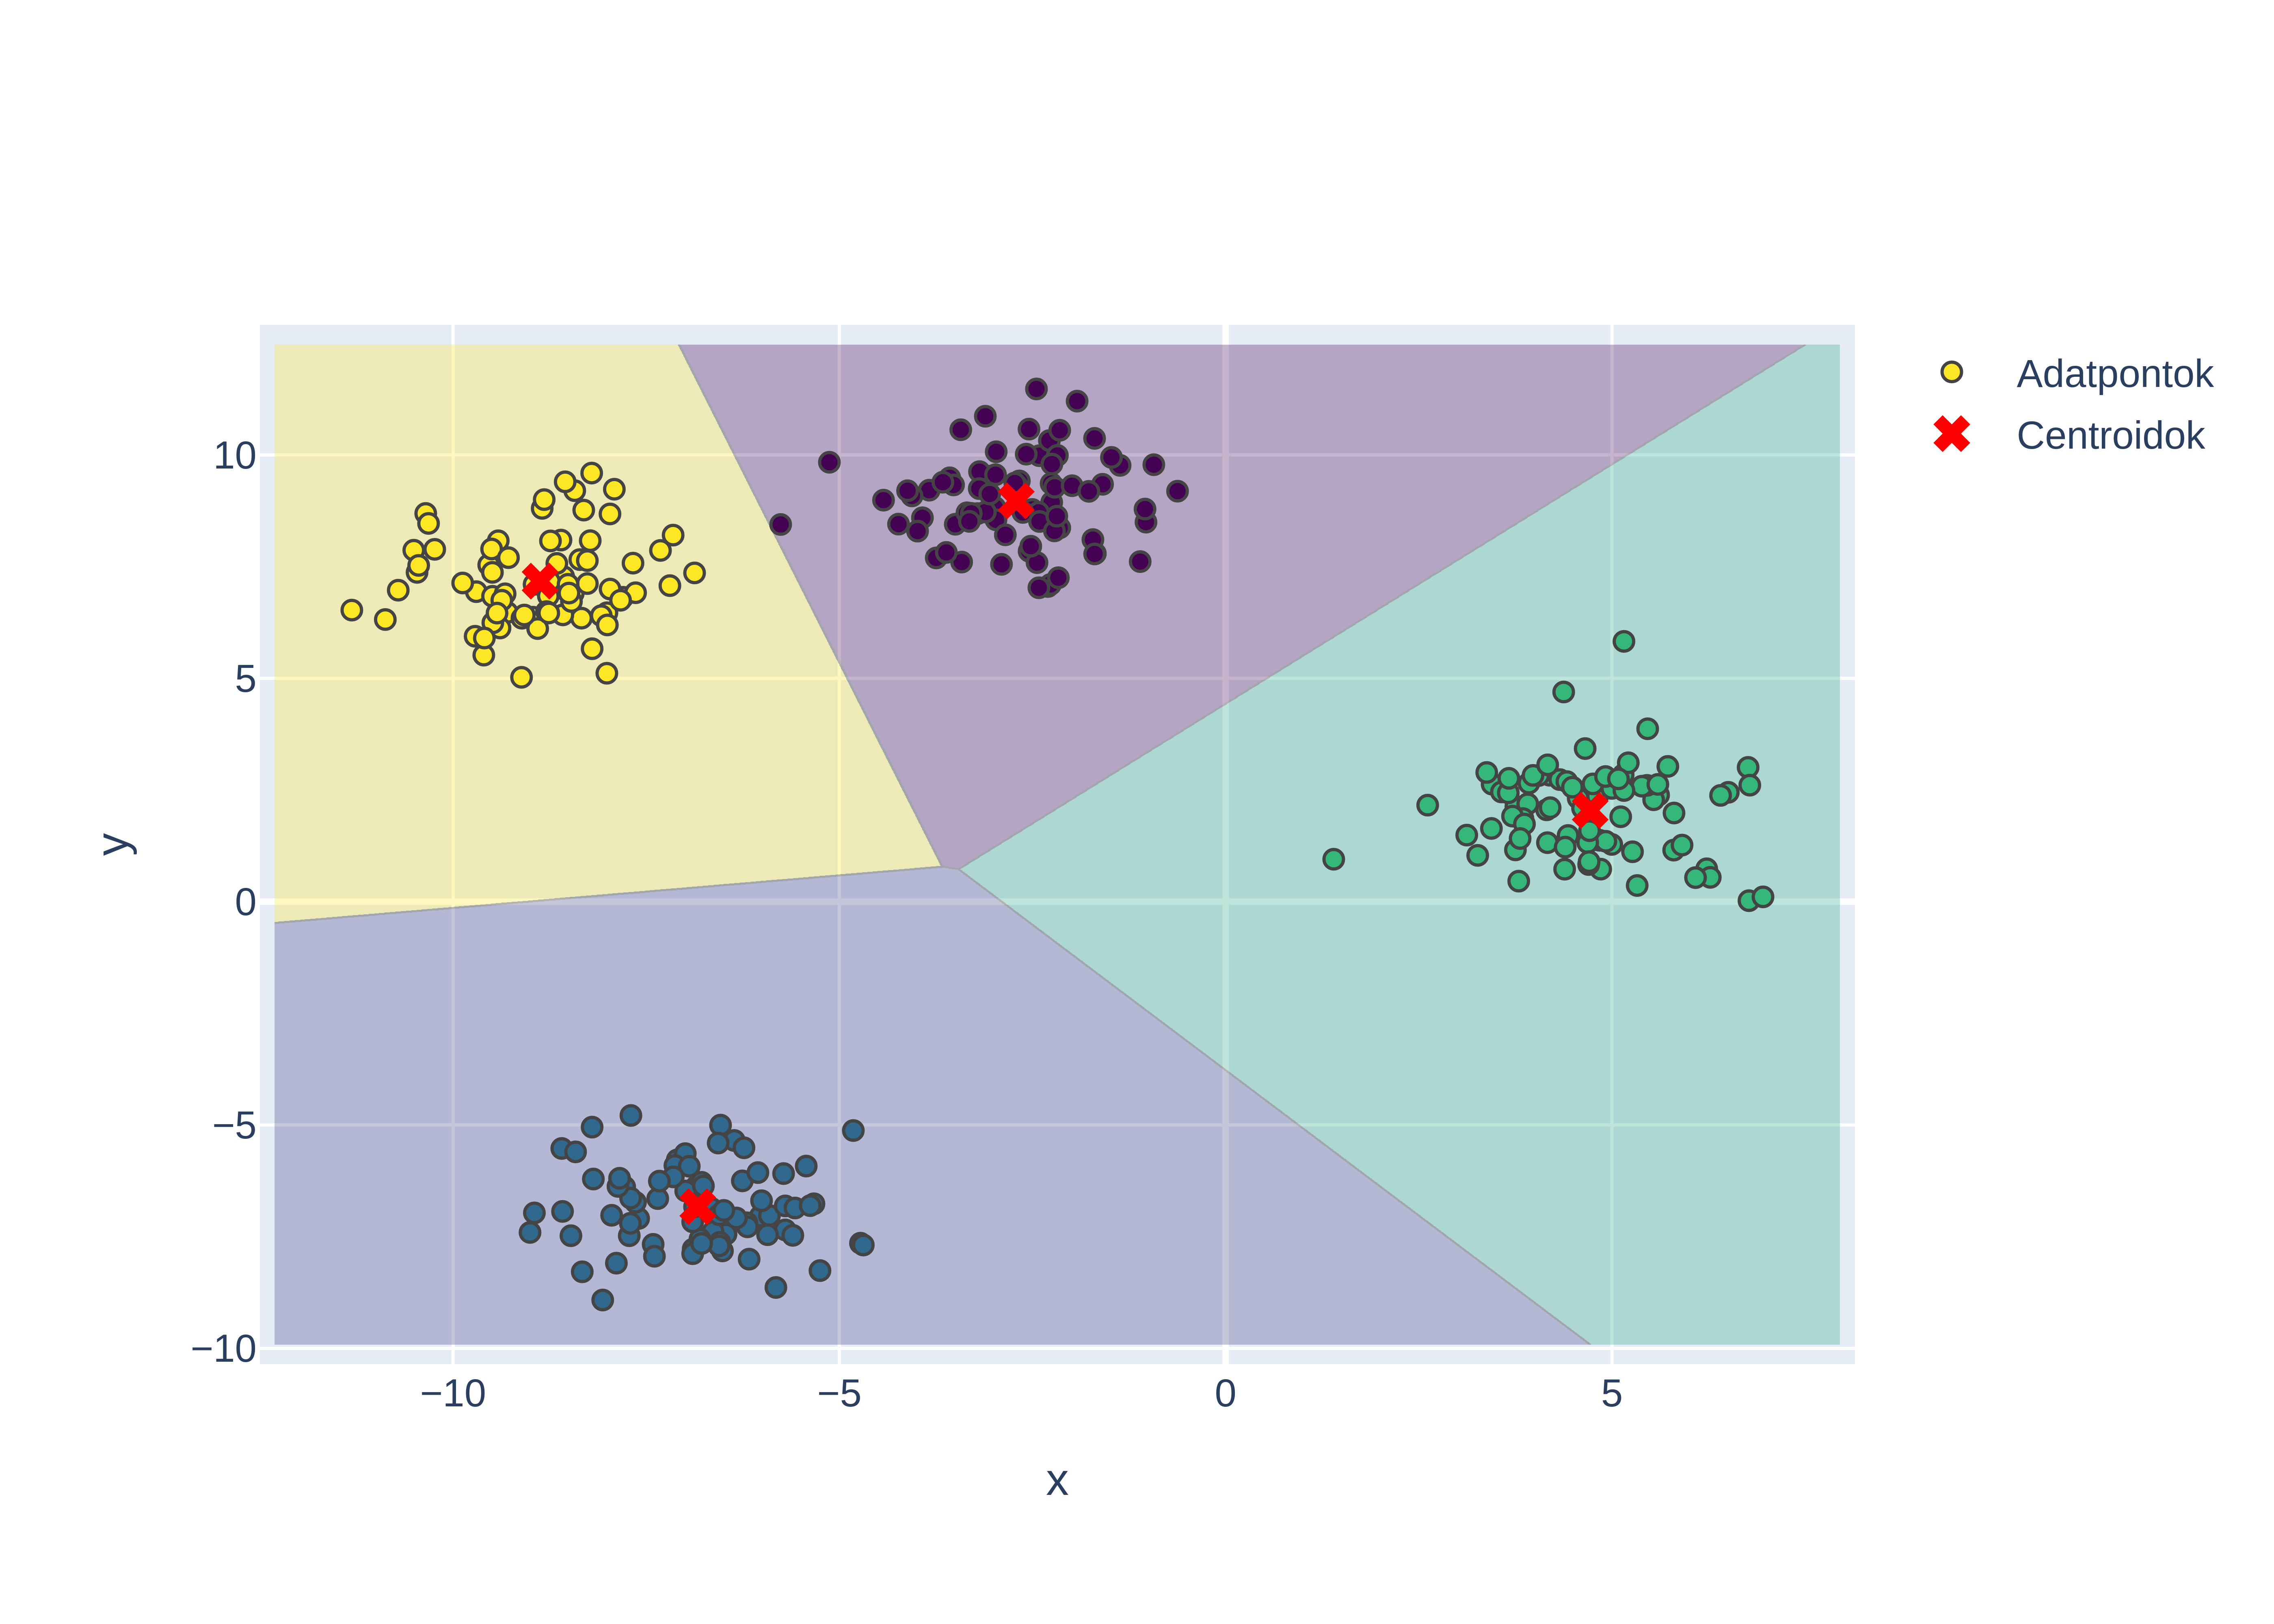
\includegraphics[width=7cm, height=7cm, keepaspectratio]{images/freq_14.png}
				\end{center}
			\end{column}
		\end{columns}
	\end{frame}
	
	\begin{frame}[fragile]{Optimális klaszterszám megtalálása}
		Egy klaszter konfiguráció annál jobb, minél szorosabban helyezkednek el az egy klaszterben lévő egyedek, és minél jobban elkülönülnek a más klaszterben lévő egyedektől. Ezt tükrözi a sziluett együttható:
		\begin{columns}
			\begin{column}{.5\textwidth}
				\begin{block}{Sziluett}
					\[
					S(x) \in \left[ -1, 1 \right]= \frac{a(x) - b(x)}{max\{ a(x), b(x)\}}
					\]
					Ahol:
					\begin{itemize}
						\item $a(x)$: $x$ mintaegyed és minden vele nem egy klaszterben lévő mintaegyed távolsága
						\item $b(x)$: $x$ mintaegyed és minden vele egy klaszterben lévő mintaegyed távolsága
					\end{itemize}
				\end{block}
			\end{column}
			\begin{column}{.5\textwidth}
				\begin{center}
					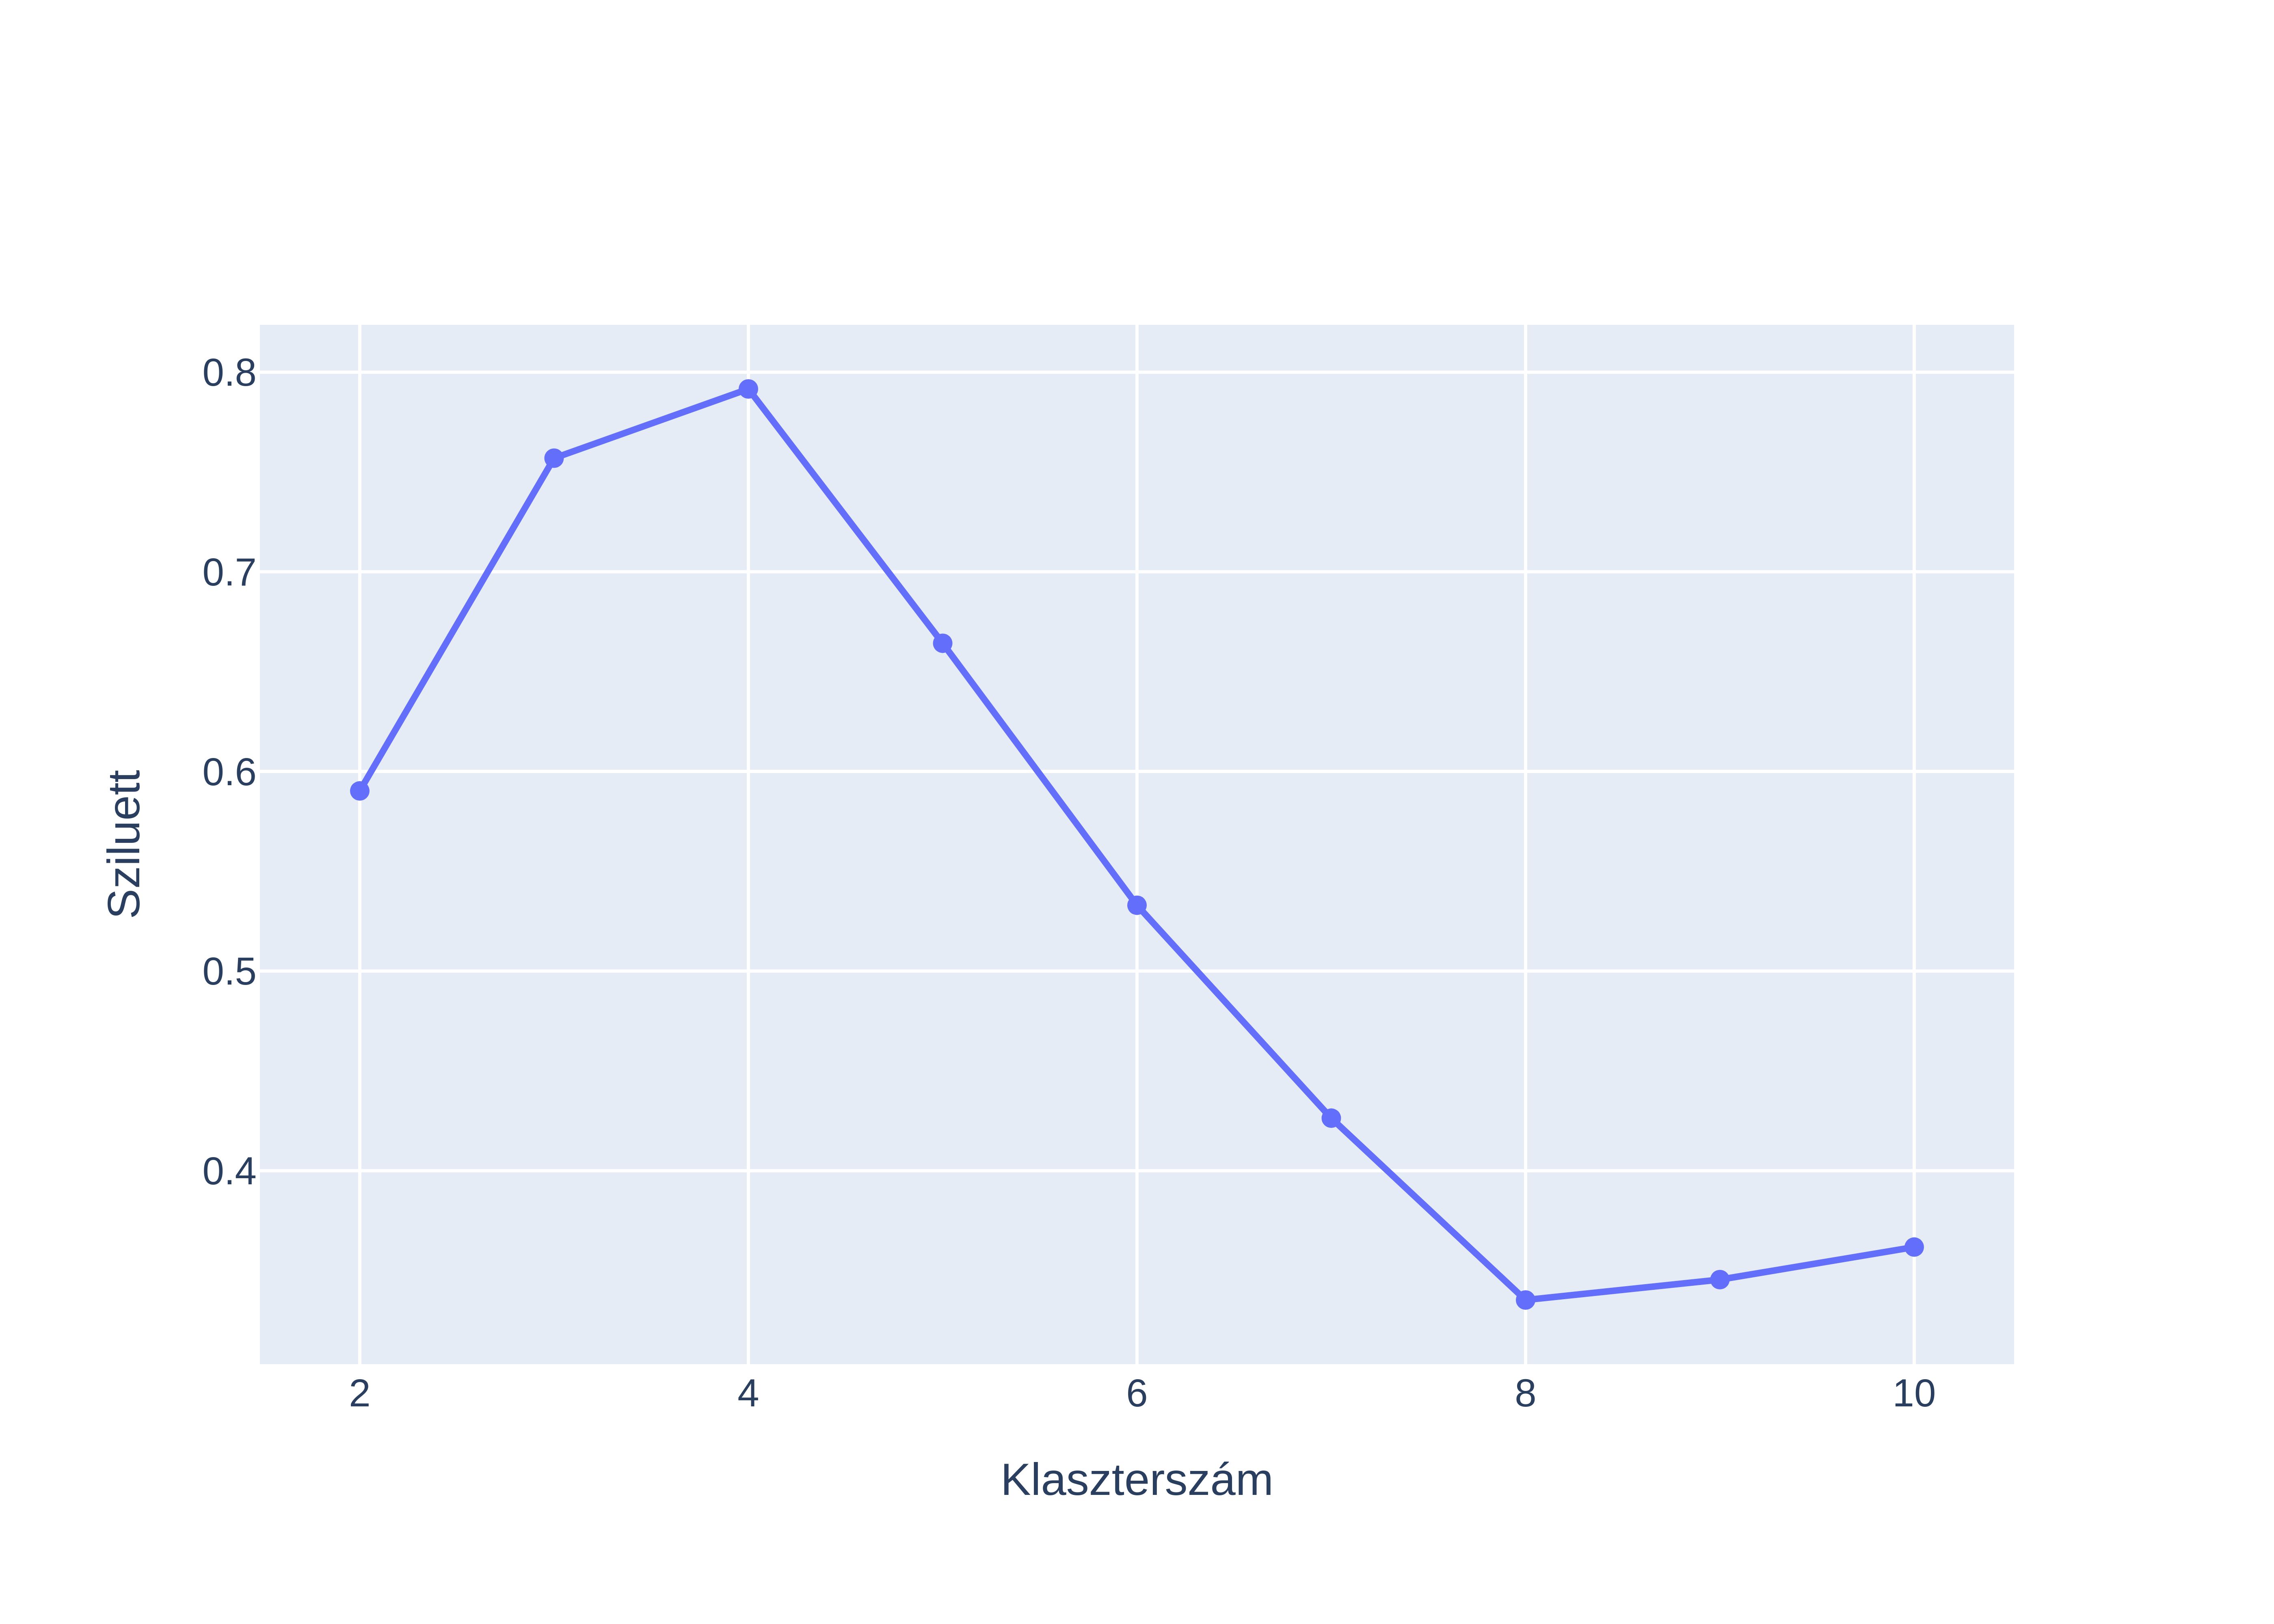
\includegraphics[width=7cm, height=7cm, keepaspectratio]{images/freq_15.png}
				\end{center}
			\end{column}
		\end{columns}
	\end{frame}
	
	\begin{frame}[fragile]{\texttt{Scikit-learn} $K$-közép }
		\begin{columns}
			\begin{column}{.5\textwidth}
				$K$-közép modul importálása és tanítása a \texttt{make\_blobs} adathalmazon:
				\begin{lstlisting}[language=python]
from sklearn.cluster import KMeans

kmeans = KMeans(n_clusters=n_clusters, random_state=random_state)
kmeans.fit(X)

labels = kmeans.labels_
centroids = kmeans.cluster_centers_
				\end{lstlisting}
			\end{column}
			\begin{column}{.5\textwidth}
				Klaszter centroidok $x$ és $y$ koordinátái:
				\begin{lstlisting}[language=python]
 In [1]: print(kmeans.cluster_centers_)
Out [1]: [[-2.70981136  8.97143336]
[-6.83235205 -6.83045748]
[ 4.7182049   2.04179676]
[-8.87357218  7.17458342]]
				\end{lstlisting}
				\par\medskip
				Becsült címkék az adathalmaz első 10 elemére:
				\begin{lstlisting}[language=python]
 In [2]: print(kmeans.labels_)
Out [2]: [3 3 0 1 3 1 2 1 0 2]
				\end{lstlisting}
			\end{column}
		\end{columns}
	\end{frame}
	
	\begin{frame}[fragile]{Országok klaszterezése}
		A következő program az országokat 5 klaszterbe sorolja be, majd ennek a kimenetét felhasználva hoz létre egy tematikus térképet:\par\smallskip
		\begin{columns}
			\begin{column}{.5\textwidth}
				\begin{lstlisting}[language=python]
year = 2018
indicators = ['Population, total']
kmeans = KMeans(n_clusters=5)
df = poverty[poverty['year'].eq(year) & poverty['is_country']]
data = df[indicators].values
kmeans.fit(data)

fig = px.choropleth(
	df,
	locations='Country Name',
	locationmode='country names',
	color=[str(x) for x in kmeans.labels_]
)	
				\end{lstlisting}
			\end{column}
			\begin{column}{.5\textwidth}
				\begin{center}
					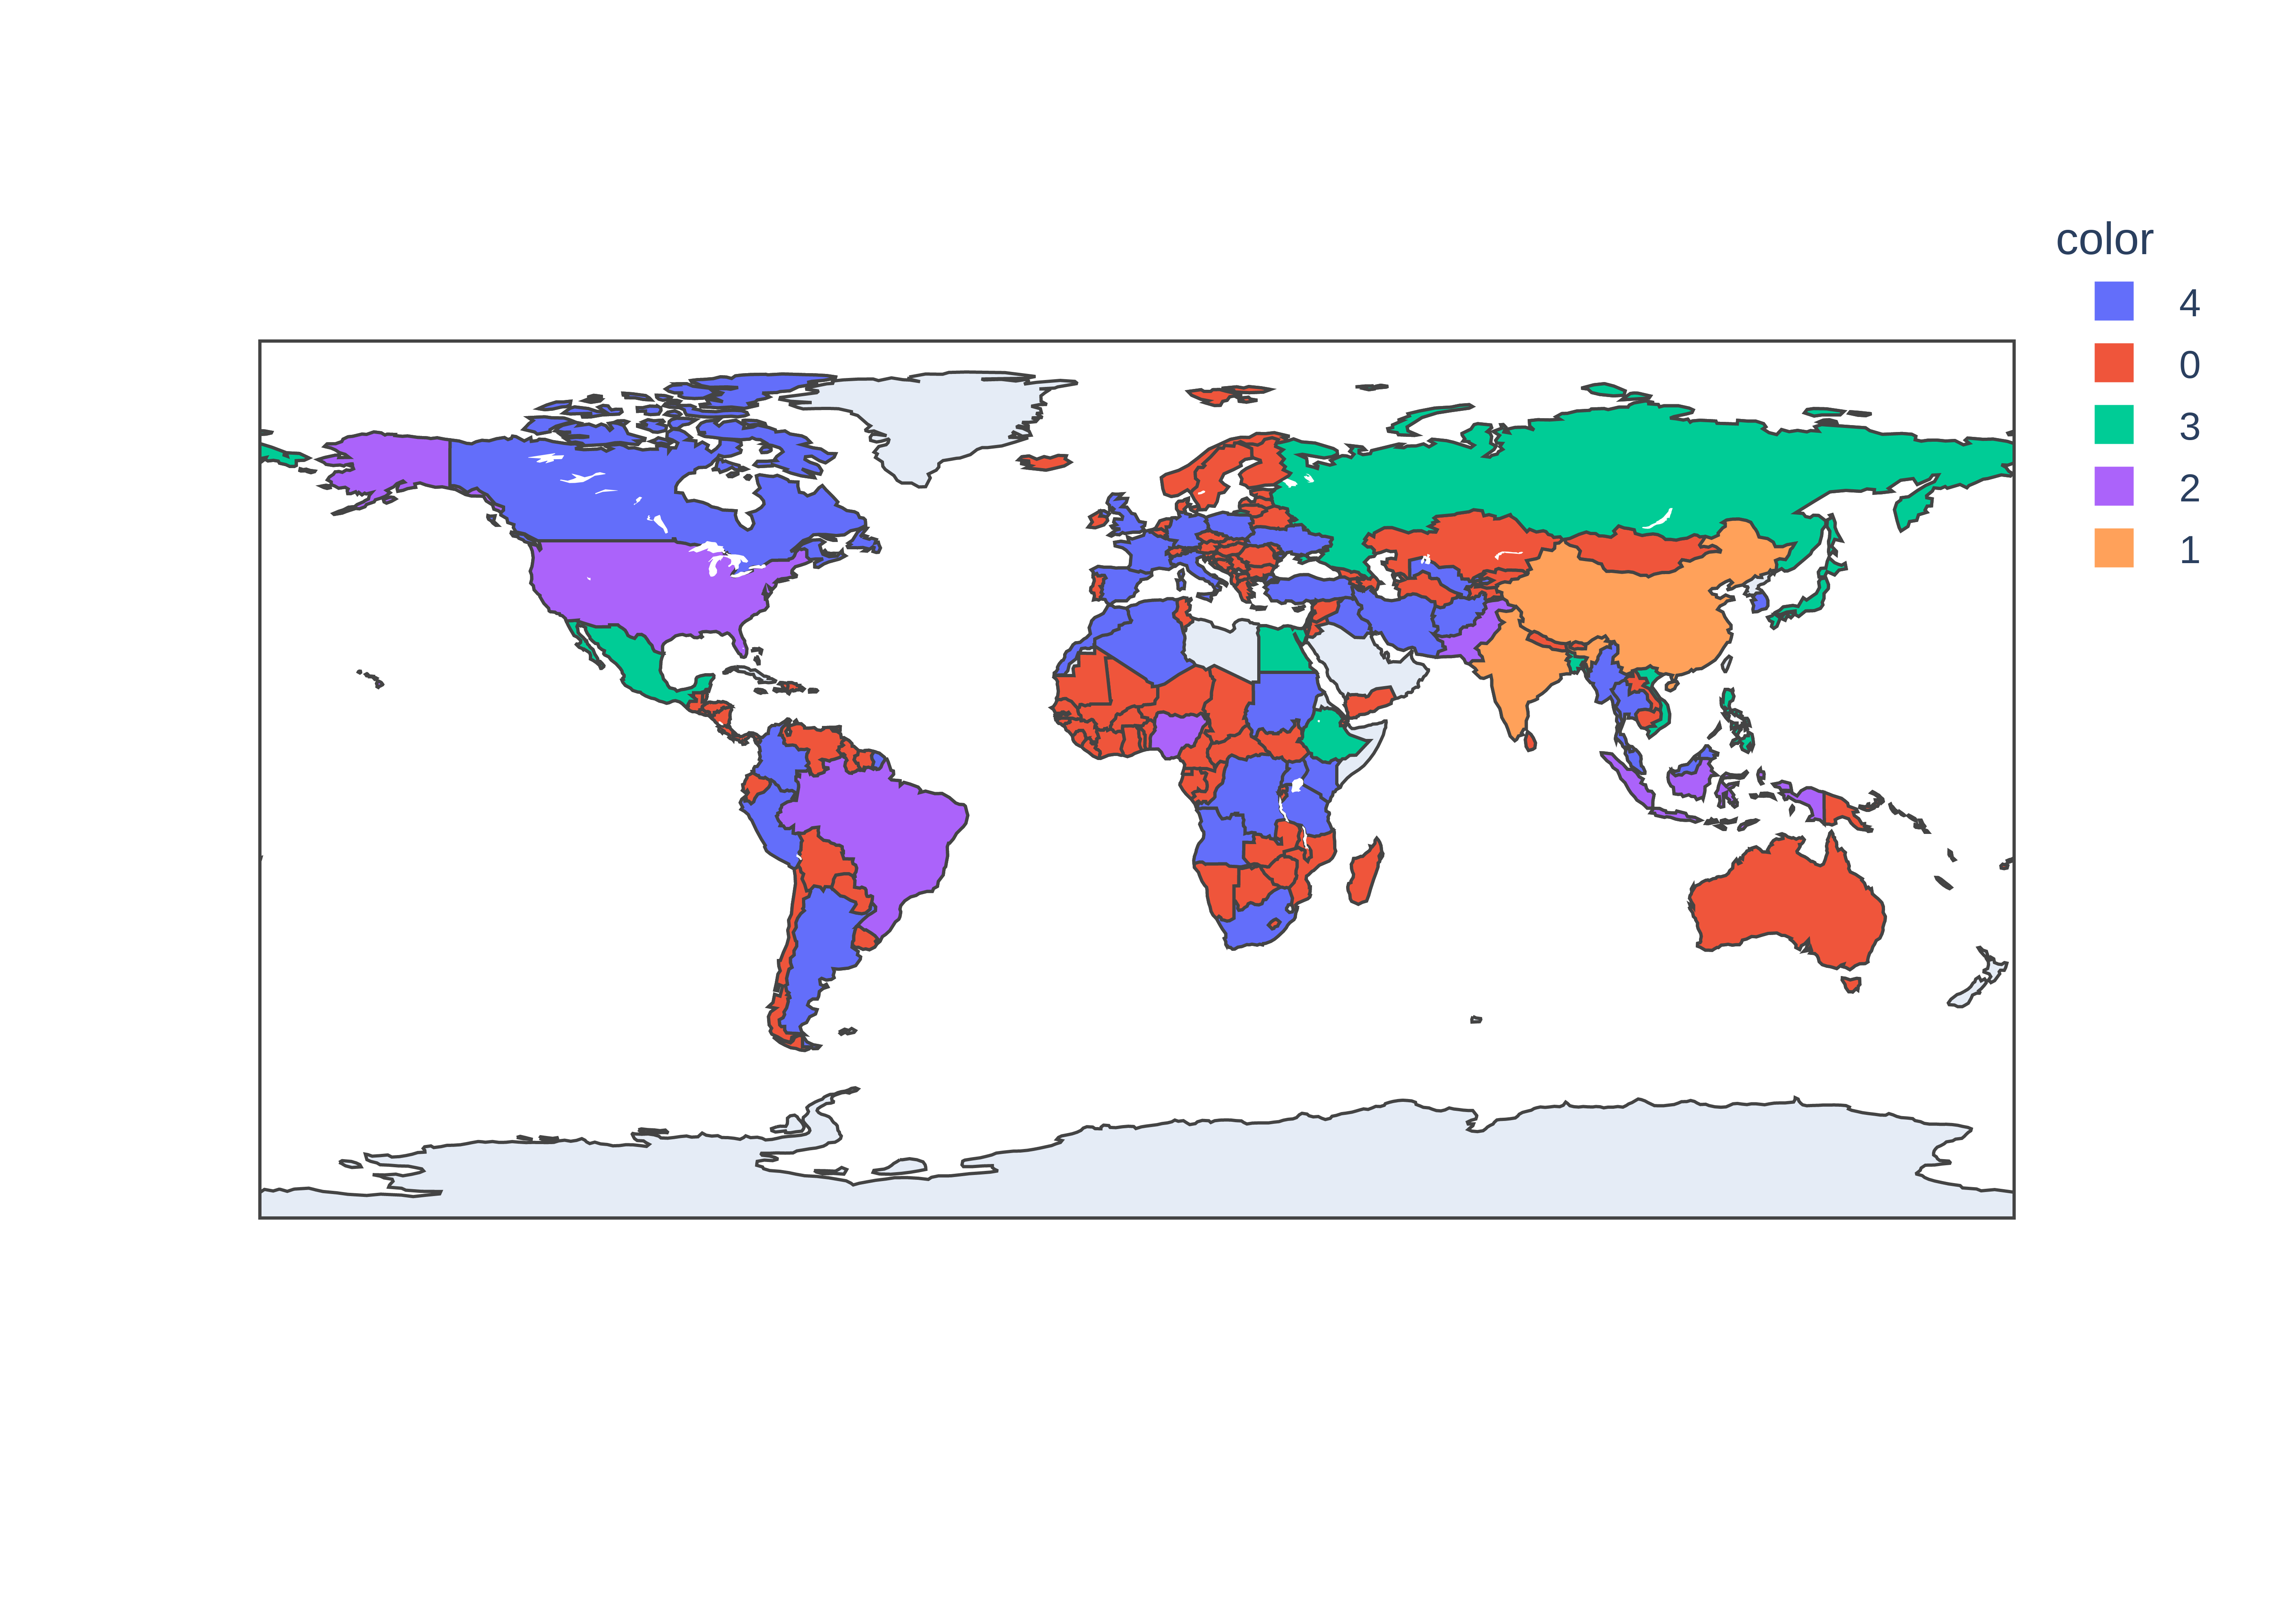
\includegraphics[width=7cm, height=7cm, keepaspectratio]{images/freq_16.png}
				\end{center}
			\end{column}
		\end{columns}
	\end{frame}
	
	\begin{frame}[fragile]{Hiányzó értékek kezelése}
		\begin{columns}
			\begin{column}{.5\textwidth}
				Az \texttt{sklearn.impute.SimpleImputer} lehetővé teszi a hiányzó értékek pótlását különböző stratégiák alkalmazásával. Néhány gyakori stratégia:
				\begin{itemize}
					\item \texttt{mean} (átlag): A hiányzó értékeket az adott oszlop átlagával helyettesíti
					\item \texttt{median} (medián): A hiányzó értékeket az adott oszlop mediánjával helyettesíti
					\item \texttt{most\_frequent} (leggyakoribb): A hiányzó értékeket az adott oszlop leggyakoribb értékével
					\item \texttt{constant} (állandó): Egy megadott állandó értékkel helyettesíti a hiányzó értékeket.
				\end{itemize}			
			\end{column}
			\begin{column}{.5\textwidth}
				\texttt{SimpleImputer}  használata:
				\begin{lstlisting}[language=python]
from sklearn.impute import SimpleImputer

data = np.array([1, 2, 1, 2, np.nan]).reshape(-1, 1)
imp = SimpleImputer(strategy='mean')
imp.fit(data)

print(imp.transform(data))
				\end{lstlisting}
				\begin{lstlisting}[language=python]
[[1. ]
[2. ]
[1. ]
[2. ]
[1.5]]
				\end{lstlisting}
			\end{column}
		\end{columns}
	\end{frame}
	
	\begin{frame}[fragile]{Adatok méretezése}
		\begin{columns}
			\begin{column}{.5\textwidth}
				\begin{lstlisting}[language=python]
from sklearn.preprocessing import StandardScaler

data = np.array([1, 2, 3, 4, 5]).reshape(-1, 1)

scaler = StandardScaler()
print(scaler.fit_transform(data))
				\end{lstlisting}
				\begin{lstlisting}[language=python]
[[-1.41421356]
[-0.70710678]
[ 0.        ]
[ 0.70710678]
[ 1.41421356]]
				\end{lstlisting}            
			\end{column}
			\begin{column}{.5\textwidth}
				\begin{block}{Méretezés}
					Adat előkészítési technika, mely során az adatok értékei egy adott tartományba transzformálódnak.
				\end{block}
				\begin{center}
					\only<1>{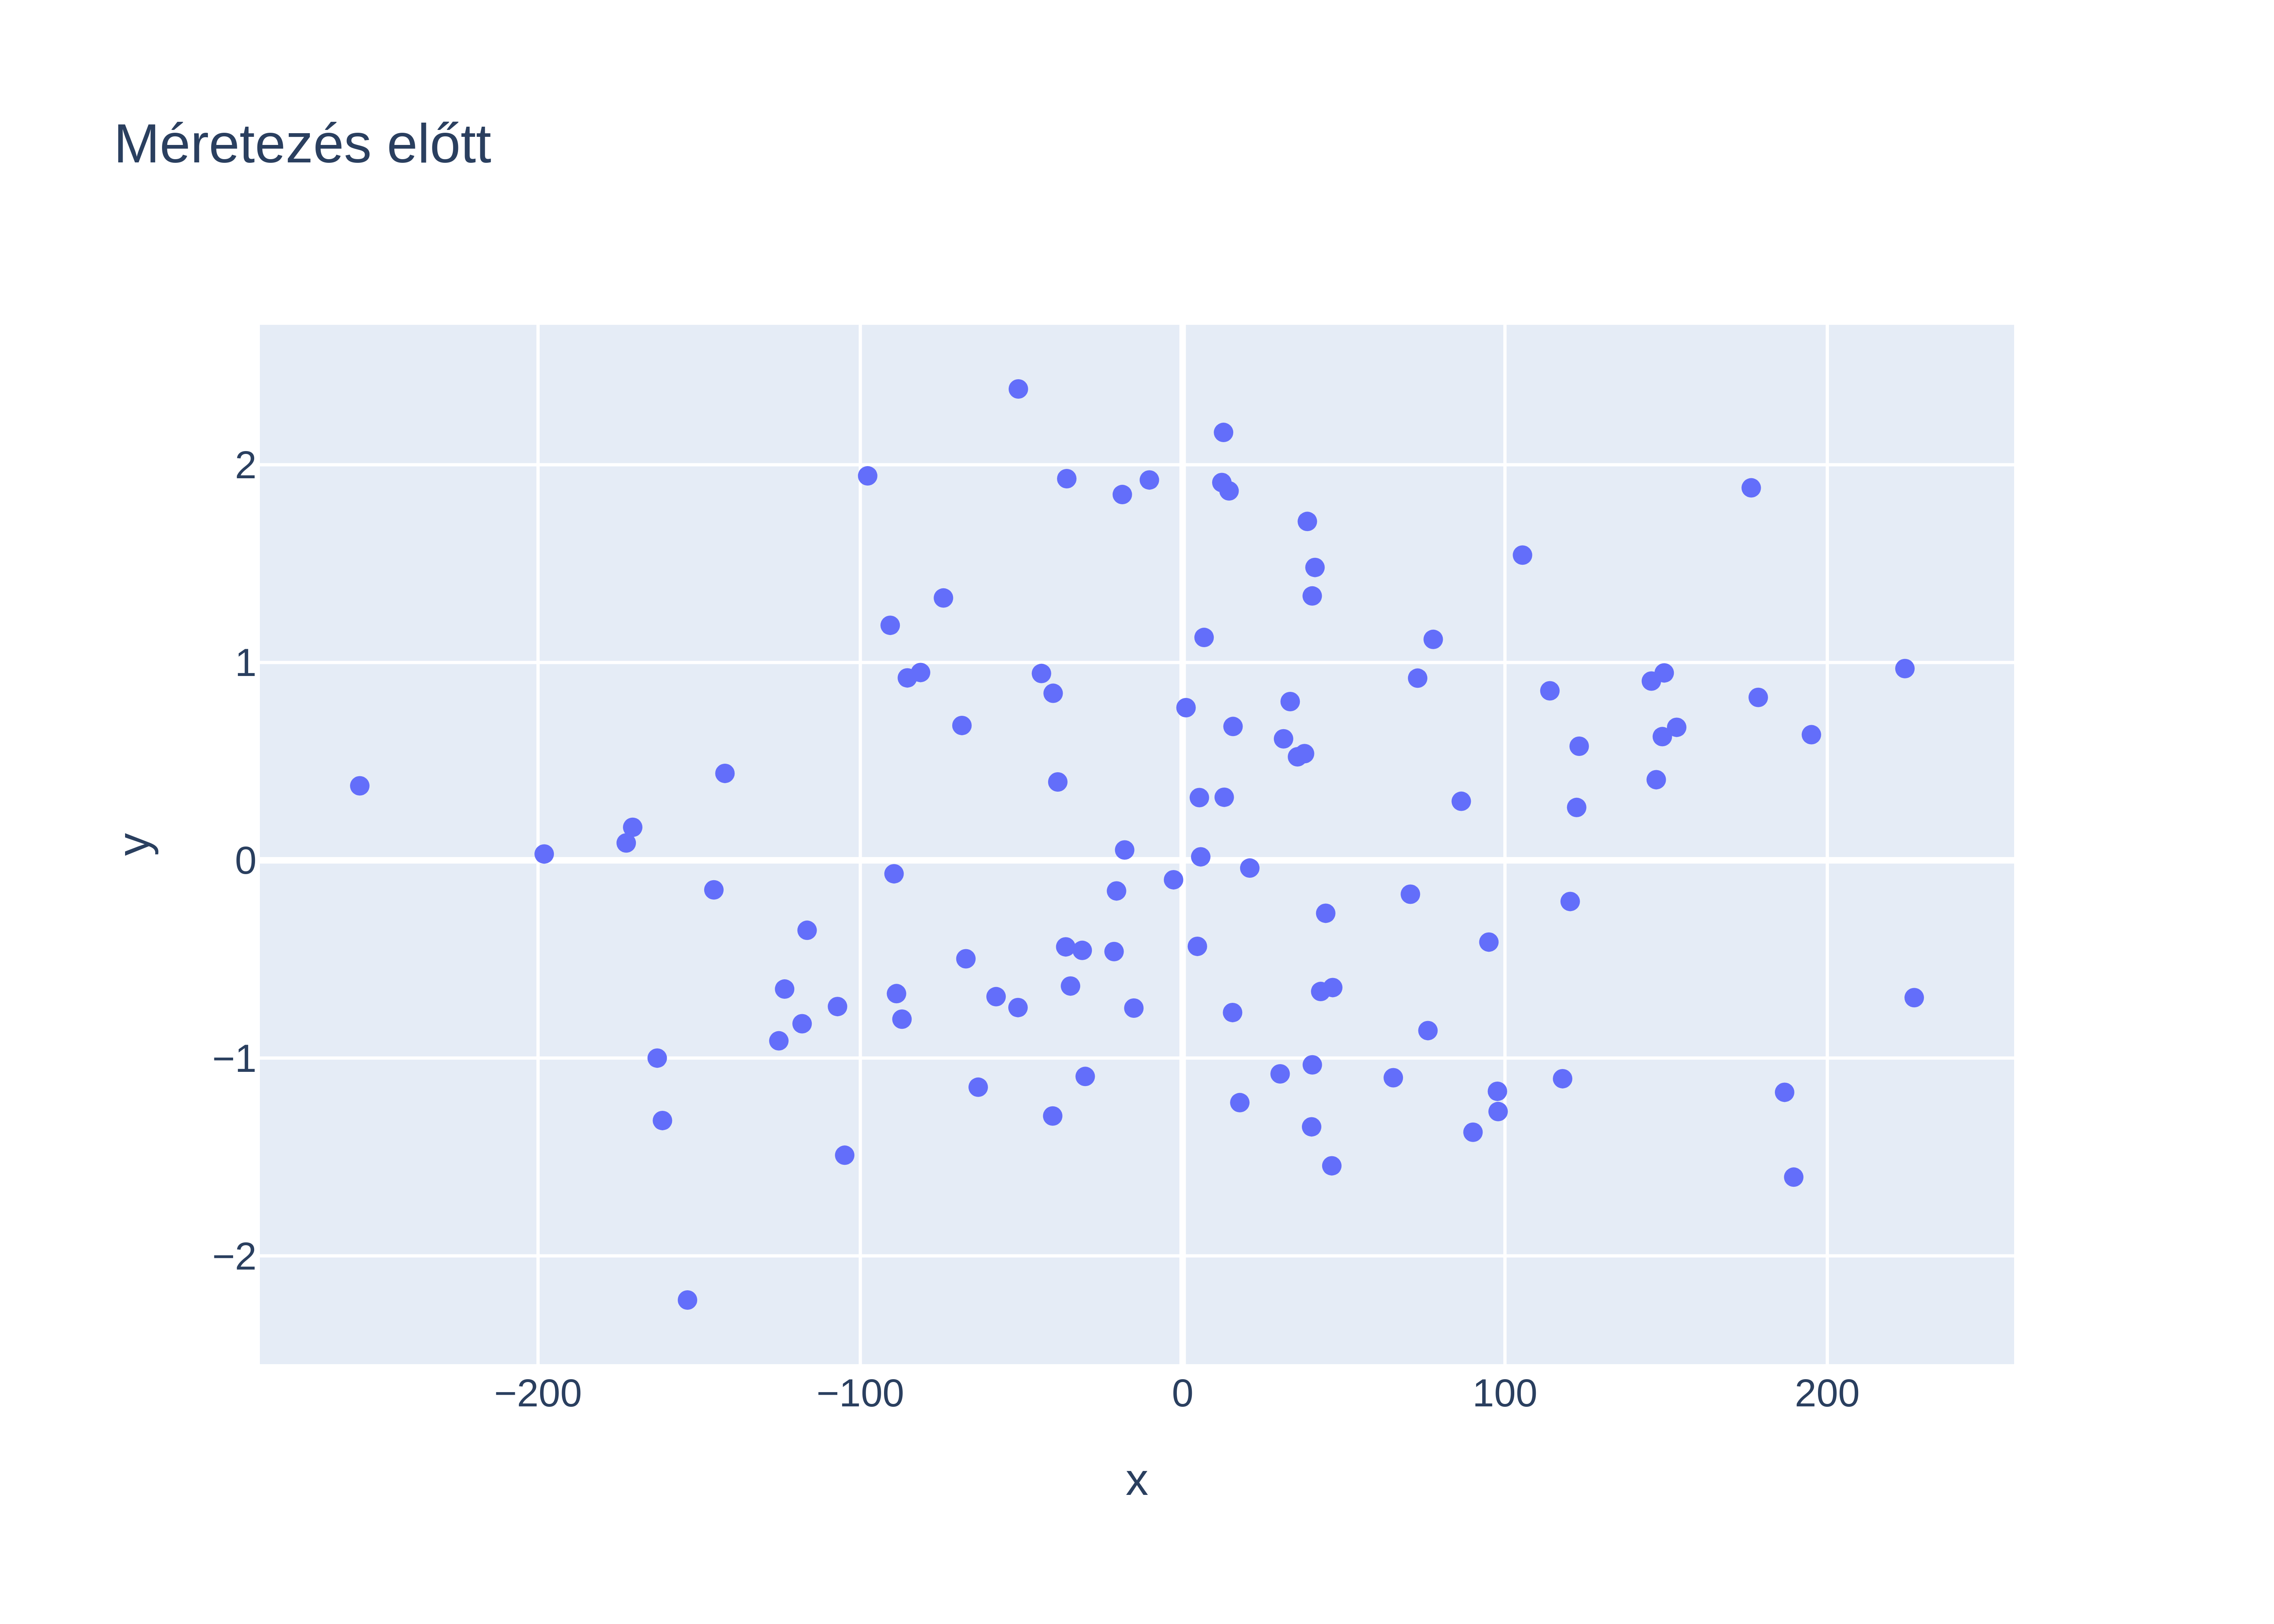
\includegraphics[width=7cm, height=7cm, keepaspectratio]{images/freq_17.png}}
					\only<2>{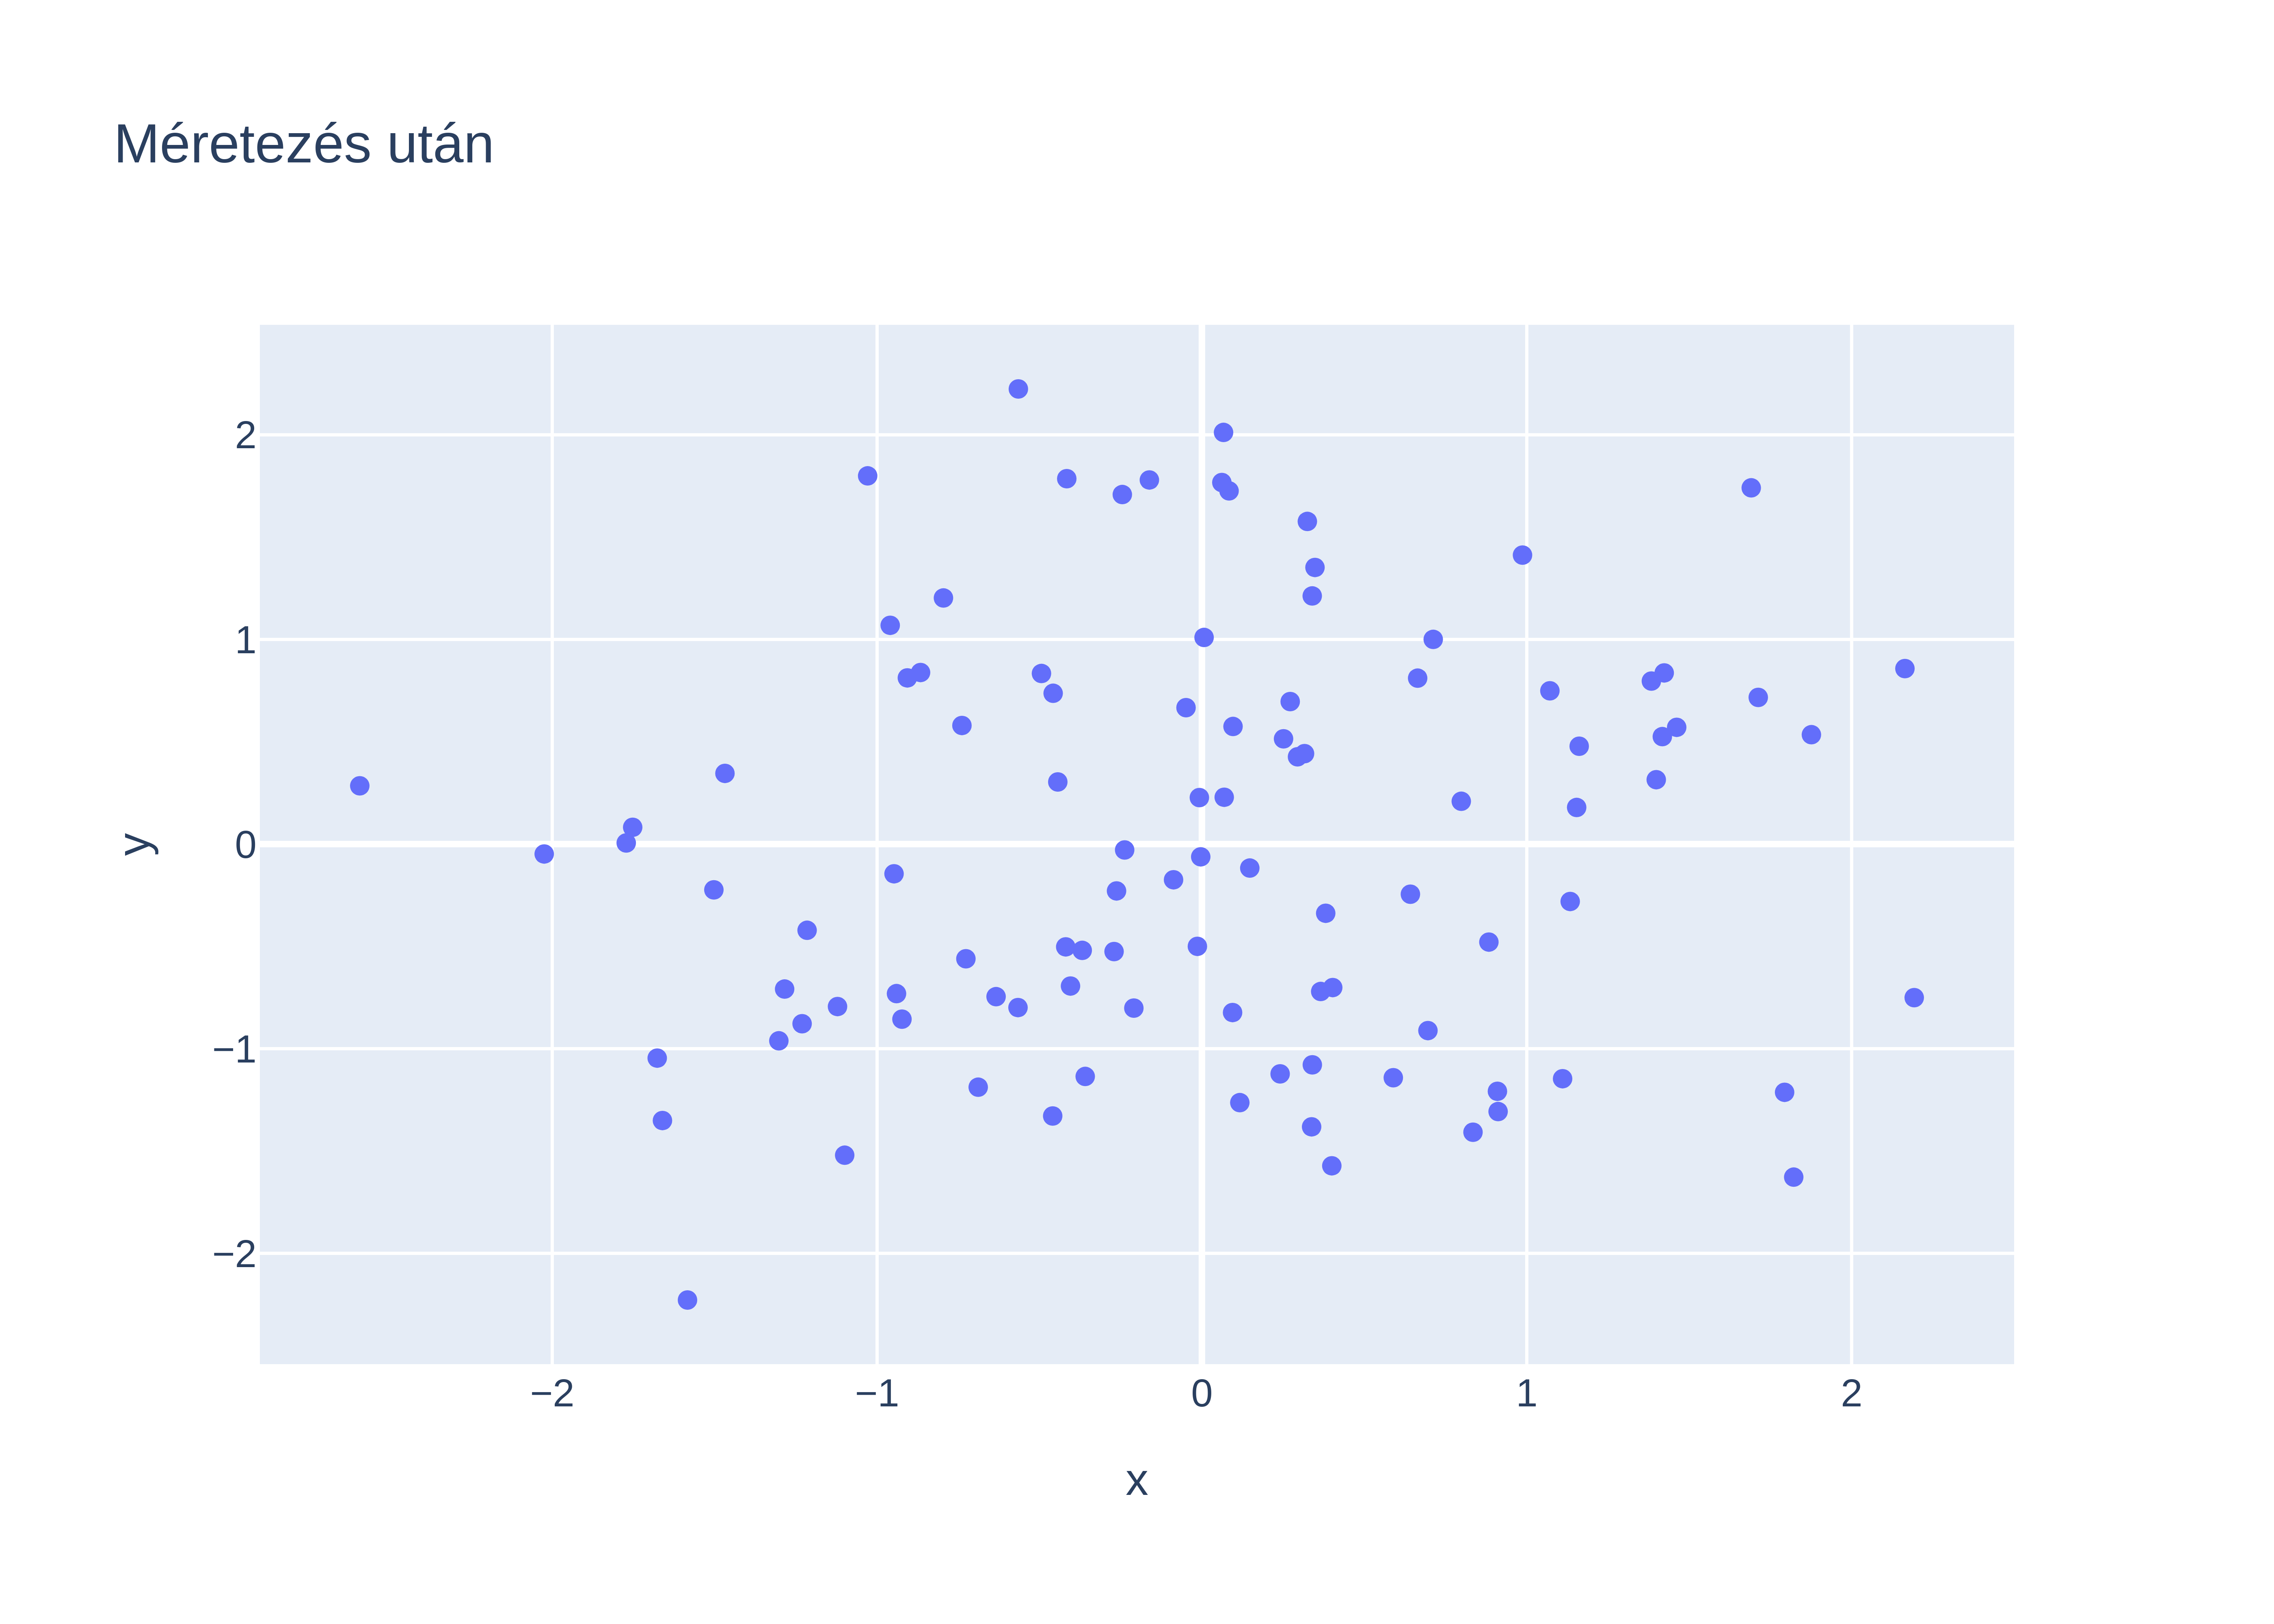
\includegraphics[width=7cm, height=7cm, keepaspectratio]{images/freq_18.png}}
				\end{center}
			\end{column}
		\end{columns}
	\end{frame}
	
	\begin{frame}{Alkalmazás interaktív térképpel, $K$-közép klaszterezéssel (\texttt{kmeans\_app.py})}
		\begin{columns}
			\begin{column}{.5\textwidth}
				A callback függvény frissíti a térképet a kiválasztott év, klaszterszám és indikátor alapján.\par\smallskip
				A hiányzó értékeket az átlaggal pótolja, majd az adatokat skálázza. A K-Közép algoritmust alkalmazza a transzformált adatokra, és a klaszterszámot a rendelkezésre álló adatok alapján korlátozza. Végül létrehozza a térképet, ahol az országokat a klaszter címkék alapján színezi, és finomhangolja a megjelenést.
			\end{column}
			\begin{column}{.5\textwidth}
				\begin{center}
					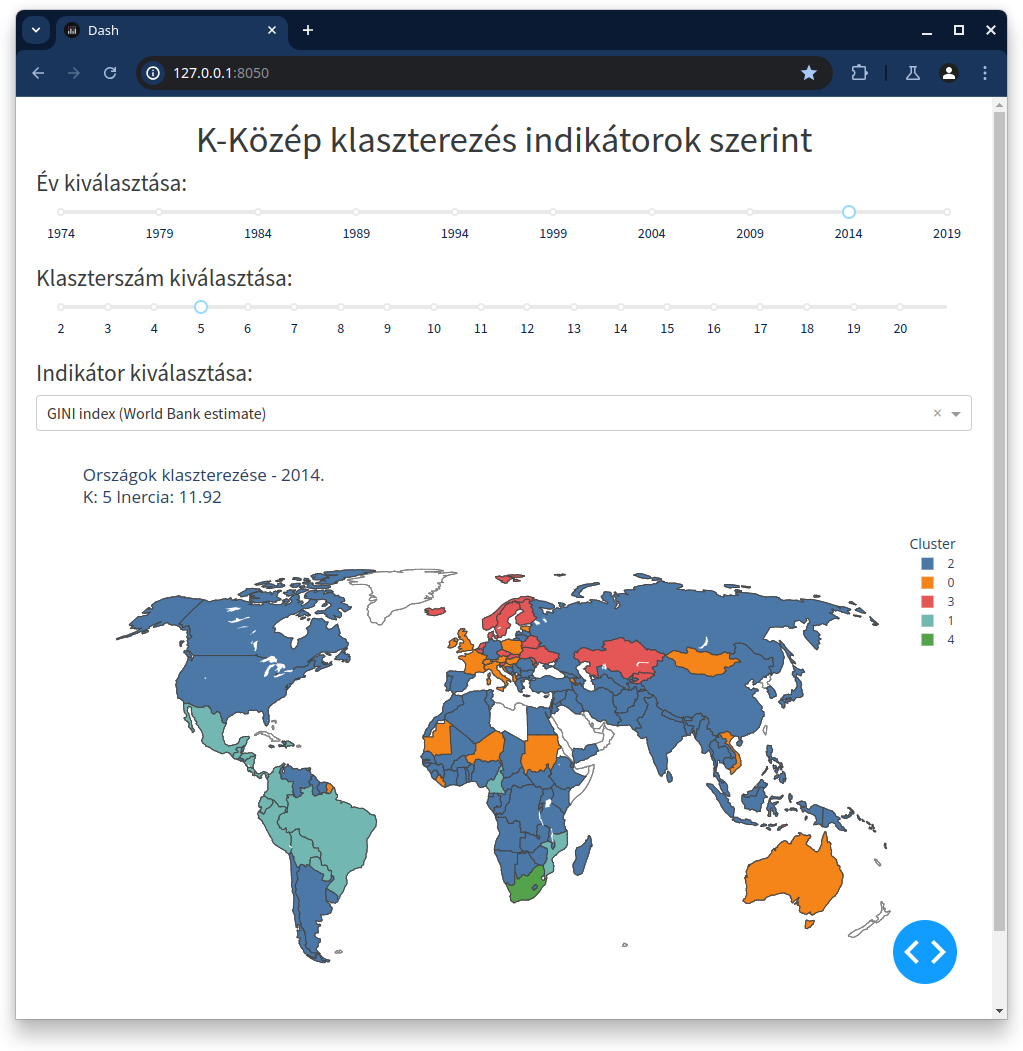
\includegraphics[width=7cm, height=7cm, keepaspectratio]{images/freq_19.png}
				\end{center}
			\end{column}
		\end{columns}
	\end{frame}
	
	\begin{frame}{$K$-közép beépítése a teljes alkalmazásba (\texttt{app\_v4\_2.py})}
		\begin{center}
			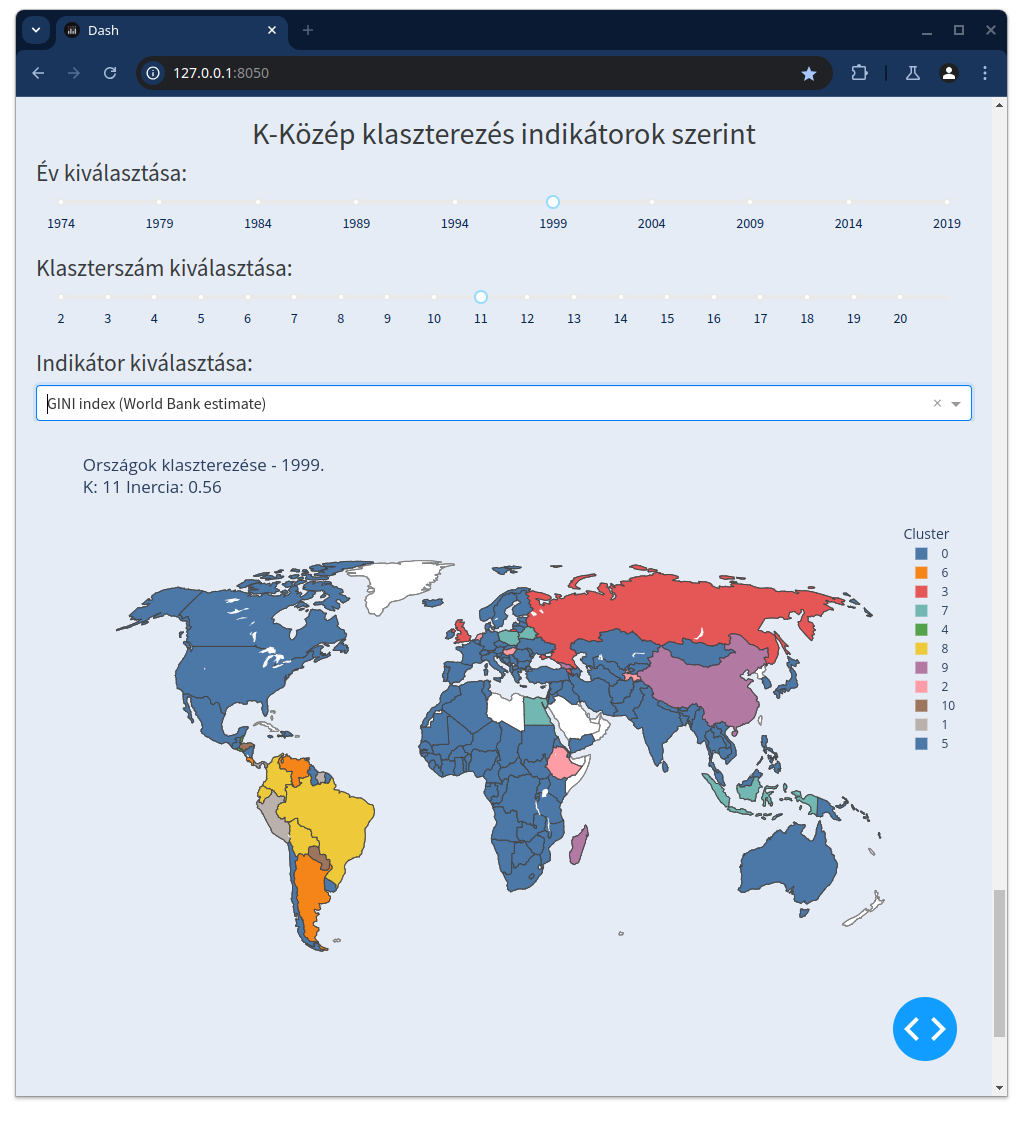
\includegraphics[width=7cm, height=7cm, keepaspectratio]{images/freq_20.png}
		\end{center}
	\end{frame}
	
	\section{Összetett callback függvények}
	
	\begin{frame}{}
		\tableofcontents[currentsection]
	\end{frame}
	
	\begin{frame}[fragile]{Komponensek állapota}
		\begin{columns}
			\begin{column}{.5\textwidth}
				Az \texttt{Output} és \texttt{Input} mellett a harmadik callback argumentum a \texttt{State}. 
				\begin{itemize}
					\item A sorrend a callback dekorátoron belül \texttt{[Input, Output, State]}.
					\item Az \texttt{Input} komponens állapotának megváltoztatása elindítja a callback függvényt, a \texttt{State} nem. 
					\item Ha egy \texttt{Input} elem módosul, a callback függvény \texttt{State} bemenő paraméterének értéke az lesz, amire az legutóbb módosult. 
				\end{itemize}
			\end{column}
			\begin{column}{.5\textwidth}
				\begin{lstlisting}[language=python]
...
html.Button('Futtatás', id='kmeans_button')
...
				\end{lstlisting}
				\begin{lstlisting}[language=python]
@app.callback(
Output('clustered_map_chart', 'figure'),
	Input('kmeans_button', 'n_clicks'),
	State('year_cluster_slider', 'value'),
	State('ncluster_slider', 'value'),
	State('indicator_dropdown', 'value'),
)
def clustered_map(n_clicks, year, n_clusters, indicator):
	if n	ot n_clicks:
		return no_update
	...
				\end{lstlisting}
			\end{column}
		\end{columns}	
	\end{frame}
	
	\begin{frame}[fragile]{Interaktív töltés indikátor}
		\begin{columns}
			\begin{column}{.5\textwidth}
				A \texttt{dcc.Loading} képes visszajelzést adni egy felhasználónak, amíg a bele ágyazott komponens frissül.\par\smallskip
				Egy diagram beágyazása \texttt{Loading} komponensbe:
				\begin{lstlisting}[language=python]
dcc.Loading([
	dcc.Graph(
		id='clustered_map_chart'
	),
])
				\end{lstlisting}
			\end{column}
			\begin{column}{.5\textwidth}
				\begin{center}
					
\includegraphics[width=3cm, height=3cm, keepaspectratio]{images/freq_21.png}
				\end{center}
			\end{column}
		\end{columns}
	\end{frame}
	
	
	\begin{frame}[fragile]{$K$-közép alkalmazás állapottal}
		\begin{columns}
			\begin{column}{.5\textwidth}
				Az alkalmazás funkcionalitásában megegyezik az előző verzióval, viszont ebben az esetben a callback függvény a Futtatás gombra kattintással indul el.\par\smallskip
				A vezérlőelemek állapota \texttt{State} argumentumon keresztül adódik át a függvénynek, ezért nem indul el az elemek állapotának módosításakor. 
			\end{column}
			\begin{column}{.5\textwidth}
				\begin{center}
					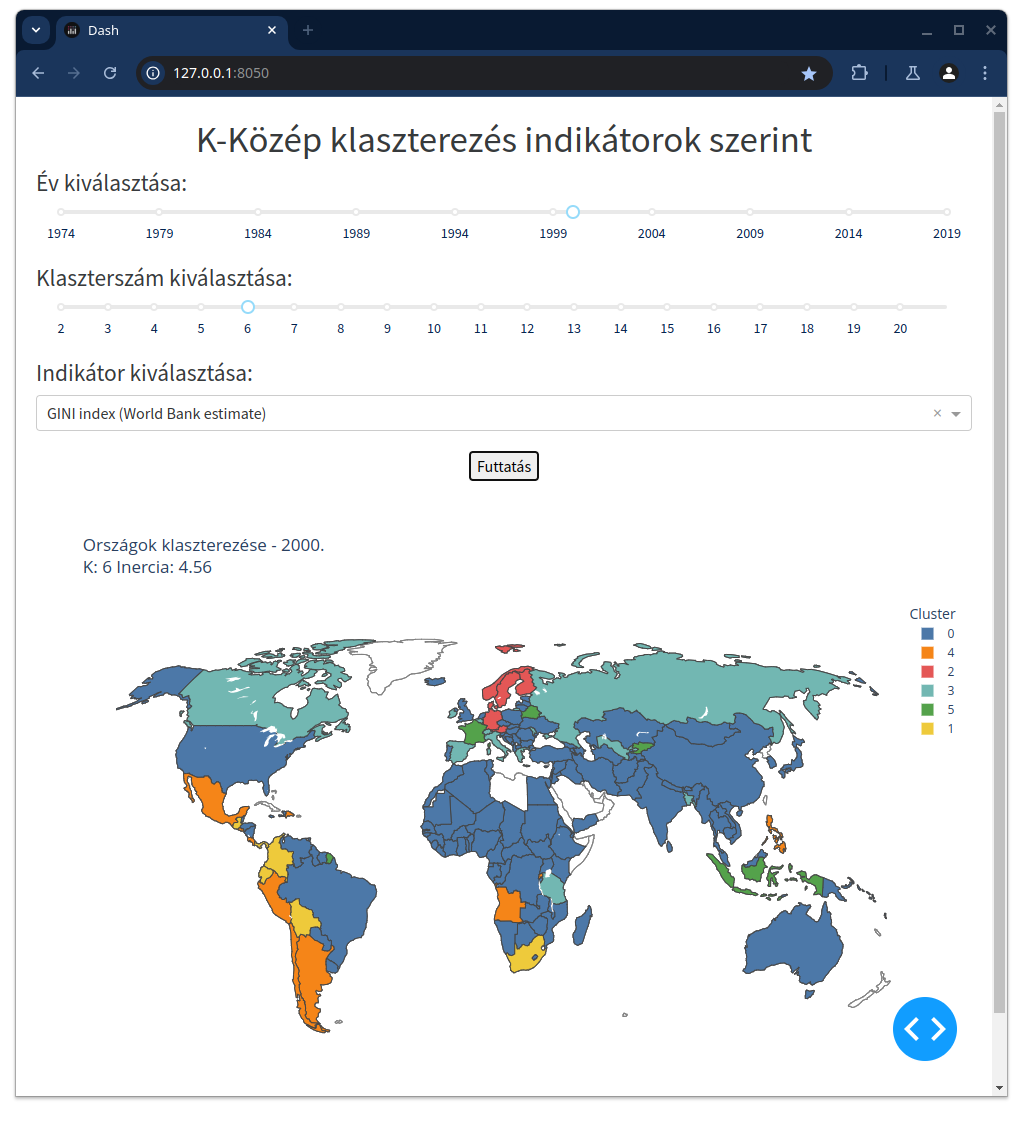
\includegraphics[width=7cm, height=7cm, keepaspectratio]{images/freq_22.png}
				\end{center}
			\end{column}
		\end{columns}
	\end{frame}
	
	\section{Komponenseket irányító komponensek}
	
	\begin{frame}{}
		\tableofcontents[currentsection]
	\end{frame}
	
	\begin{frame}{Komponensvezérlő alkalmazás (\texttt{component\_app\_v1.py})}
		\begin{columns}
			\begin{column}{.5\textwidth}
				\begin{itemize}
					\item \textbf{Elrendezés}: Az alkalmazás HTML és Dash komponensekből épül fel, beleértve információs üzenetet, egy szövegmezőt, gombot, legördülő menüt és grafikont.
					\item \textbf{Callback függvények:}
					\begin{itemize}
						\item \textbf{Legördülő menü frissítése}: A gomb megnyomására frissíti a legördülő menü opcióit a szövegmező tartalma alapján, és visszajelző üzenetet jelenít meg.
						\item \textbf{Diagram frissítése}: A legördülő menü kiválasztott értéke alapján frissíti a népesség diagramot.
					\end{itemize}
				\end{itemize}
			\end{column}
			\begin{column}{.5\textwidth}
				\begin{center}
					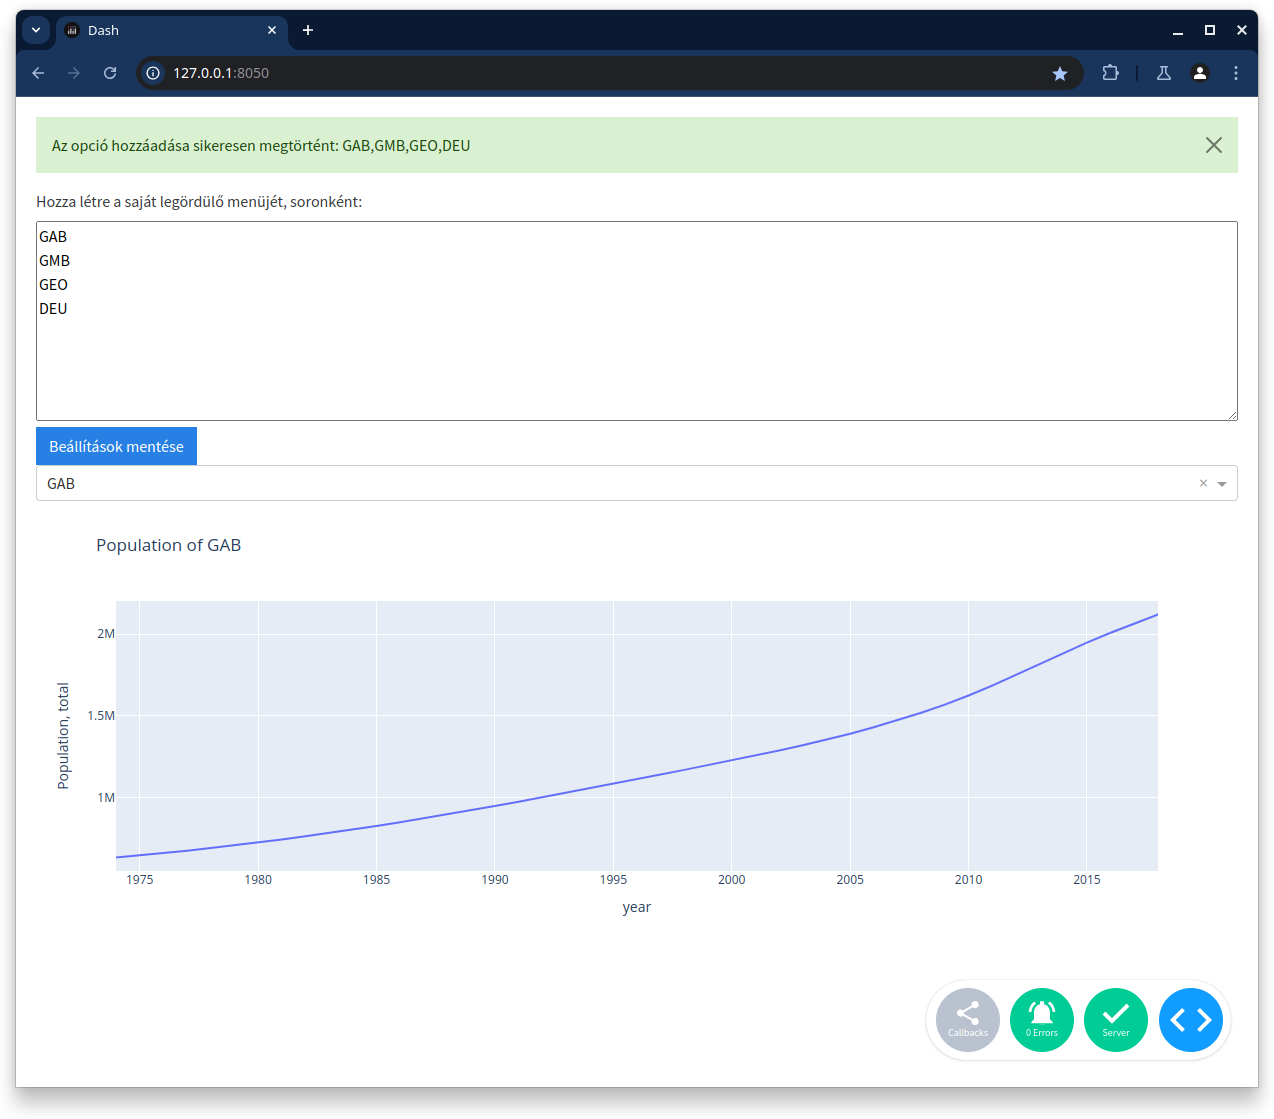
\includegraphics[width=7cm, height=7cm, keepaspectratio]{images/freq_23.png}
				\end{center}	
			\end{column}
		\end{columns}
	\end{frame}
	
	\begin{frame}[fragile]{Információs üzenetek}
		\begin{columns}
			\begin{column}{.5\textwidth}
				A \texttt{dbc.Alert} információs üzenetek megjelenítésére használhatunk a Dash alkalmazásokban:
				\begin{itemize}
					\item \texttt{primary}: Információ kék színnel
					\item \texttt{danger}: Figyelmeztetés piros színnel
					\item \texttt{success}: Siker zöld színnel
				\end{itemize}
				\par\medskip
				\texttt{Div} definiálása az elrendezésben:
				\begin{lstlisting}[language=python]
app.layout = html.Div([
	...
	html.Div(id='component_feedback'),
	...
])
				\end{lstlisting}
			\end{column}
			\begin{column}{.5\textwidth}
				Callback függvény ami a \texttt{Div.children} attribútumot módosítja: 
				\begin{lstlisting}[language=python]
@app.callback(
	Output('component_feedback', 'children')
)
def set_feedback():
	return dbc.Alert(
		f"Az opció hozzáadása sikeresen megtörtént: {','.join(text)}",
		color='success',
		dismissable=True,
	)
				\end{lstlisting}
				\par\smallskip
				\begin{center}
					
\includegraphics[width=7cm, height=7cm, keepaspectratio]{images/freq_25.png}
				\end{center}
			\end{column}
		\end{columns}
	\end{frame}
	
	\begin{frame}[fragile]{Elrendezés létrehozása}
		\begin{columns}
			\begin{column}{.5\textwidth}
				\begin{enumerate}
					\item \texttt{Div} létrehozása az üzenetnek:
					\begin{lstlisting}[language=python]
html.Div(id='component_feedback'),
					\end{lstlisting}
					\item \texttt{dcc.TextArea} szövegdoboz:
					\begin{lstlisting}[language=python]
dcc.Textarea(
	id='component_text',
	cols=40,
	rows=5,
	style={'width': '100%', 'height': 200},
),
					\end{lstlisting}
				\end{enumerate}
			\end{column}
			\begin{column}{.5\textwidth}
				\begin{enumerate}
					\setcounter{enumi}{2}
					\item Gomb, ami a callback függvényt indítja:
					\begin{lstlisting}[language=python]
dbc.Button('Beállítások mentése', id='component_button'),
					\end{lstlisting}
					\item Legördülő lista:
					\begin{lstlisting}[language=python]
dcc.Dropdown(id='component_dropdown'),
					\end{lstlisting}
					\item Grafikon:
					\begin{lstlisting}[language=python]
dcc.Graph(id='component_chart'),
					\end{lstlisting}
				\end{enumerate}
			\end{column}
		\end{columns}
	\end{frame}
	
	\begin{frame}[fragile]{Legördülő menü frissítése}
		\begin{columns}
			\begin{column}{.4\textwidth}
				A függvény a \texttt{component\_button} gomb megnyomására indul, és állapotként a szövegmező aktuális értékét fogadja.\par\smallskip
				A szövegmező tartalmát a logika felbontja szóközök mentén különálló szavakra, majd egy sikeres visszajelző üzenettel tér vissza azáltal, hogy a \texttt{component\_feedback} \texttt{Div} állapotát változtatja meg.\par\smallskip
				Az új opciókat egy listába rendezi, majd visszatér az új legördülő menü opciókkal és a diagrammal. 
			\end{column}
			\begin{column}{.6\textwidth}
				\begin{lstlisting}[language=python]
@app.callback(
	Output('component_dropdown', 'options'),
	Output('component_feedback', 'children'),
	Input('component_button', 'n_clicks'),
	State('component_text', 'value')
)
def set_dropdown_options(n_clicks, options):
	if not n_clicks:
		return no_update
	text = options.split()
	message = dbc.Alert(
		f"Az opció hozzáadása sikeresen megtörtént: {','.join(text)}",
		color='success',
		dismissable=True
	)
	options = [{'label': t, 'value': t} for t in text]
	return options, message
				\end{lstlisting}
			\end{column}
		\end{columns}
	\end{frame}
	
	\begin{frame}[fragile]{Diagram frissítése}
		\begin{columns}
			\begin{column}{.5\textwidth}
				A függvény a \texttt{component\_chart}  legördülő menü kiválasztott értékét (\texttt{country\_code}) veszi bemenetként. Ha nincs kiválasztott érték a diagram nem frissül.\par\smallskip
				A \texttt{poverty} adatkészlet szűrése után létrehoz egy vonaldiagramot, amely az adott ország népességének változását mutatja meg az évek során.
			\end{column}
			\begin{column}{.5\textwidth}
				\begin{lstlisting}[language=python]
@app.callback(
	Output('component_chart', 'figure'),
	Input('component_dropdown', 'value')
)
def create_population_chart(country_code):
	if not country_code:
		return no_update
	# Adatkészlet szűrése
	df = poverty[poverty['Country Code'] == country_code]
	# Diagram létrehozása
	return px.line(
		df,
		x='year',
		y='Population, total',
		title=f"Population of {country_code}"
	)
				\end{lstlisting}
			\end{column}
		\end{columns}
	\end{frame}
	
	\begin{frame}{Az alkalmazás callback gráfja}
		\begin{columns}
			\begin{column}{.5\textwidth}
				A callback gráf vizuálisan ábrázolja a különböző komponensek közötti kapcsolatokat, segít lekövetni felhasználói események sorozatait balról elindulva a nyilak mentén, és hogy melyik komponens melyik attribútuma indította el a folyamatot.\par\medskip 
				Ez megkönnyíti a Dash alkalmazásokban való hibakeresést. 
			\end{column}
			\begin{column}{.5\textwidth}
				\begin{center}
					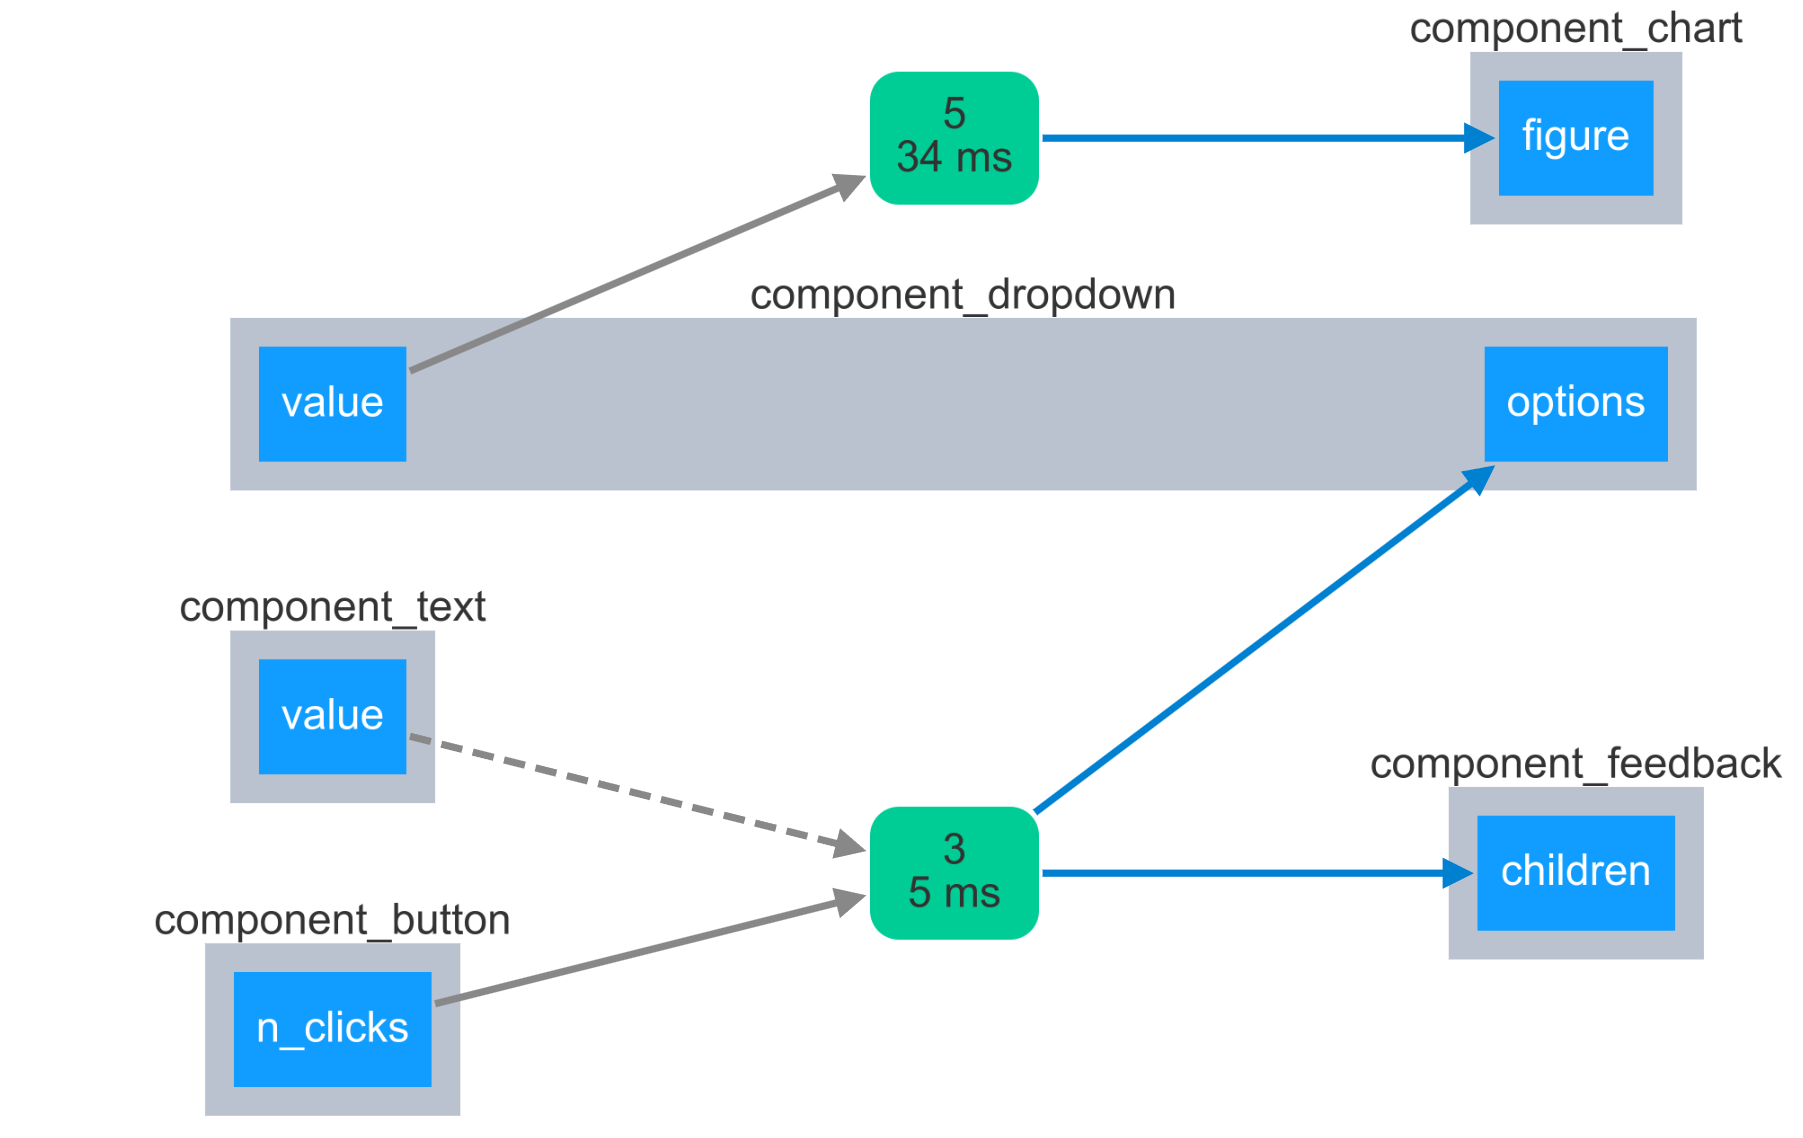
\includegraphics[width=7cm, height=7cm, keepaspectratio]{images/freq_24.png}
				\end{center}
			\end{column}
		\end{columns}
	\end{frame}
\end{document}